\documentclass[14pt, table]{extarticle}
\usepackage{amsfonts}
\usepackage{amsmath}
\usepackage[utf8]{inputenc}
\usepackage[a4paper, total={7in, 10.5in}]{geometry}
\usepackage[table]{xcolor}
\usepackage{tgbonum}
\usepackage{float}
\usepackage{graphicx}
\graphicspath{ {./images/} }
\DeclareGraphicsExtensions{.png,.jpg}
\usepackage{caption}
\usepackage{tikz}
\usepackage{circuitikz}
\usepackage[T1]{fontenc}
\usetikzlibrary{quotes,angles}
\usetikzlibrary{arrows}
\usetikzlibrary{circuits.logic.US}
\usetikzlibrary{positioning}
\hyphenpenalty 5000
\usepackage{subfig}
\usepackage{array}

\title{\textbf{Sprawozdanie} \\ \Large{Ćwiczenie 4}}
\date{Data wykonania: 10 maja 2023}
\author{ \Large{Jan Kwinta, grupa 12} \\ \large{Prowadzący ćwiczenia: dr. Szymon Niedźwiedzki}}


\newcommand{\nl}{\vspace{0.5cm}}
\newcommand{\nz}{\vspace{1.5cm}}

\begin{document}
\maketitle

\paragraph{Wstęp \\}
Na czwartych laboratoriach z elektroniki cyfrowej montowaliśmy proste układy cyfrowe przy pomocy układów scalonych TTL (ang. \textit{transistor-transistor logic}). Główną częścią układów TTL są bramki logiczne: w przypadku tego ćwiczenia dwuwejściowe bramki NAND, NOR oraz XOR. Bramki NAND i NOR są najbardziej uniwersalnymi bramkami, za pomocą tylko bramek NAND albo tylko bramek NOR można zbudować układ realizujący dowolną funkcję logiczną algebry Boole'a. \\

\paragraph{NAND \\}
Bramka NAND z wejściami \textit{A} i \textit{B} realizuje funkcję NOT-AND, czyli 

$$ NOT \ ( \ \textit{A} \ AND \ \textit{B} \ ) $$

\nl
Oznaczenie bramki NAND w schematach układów logicznych:
\begin{center}
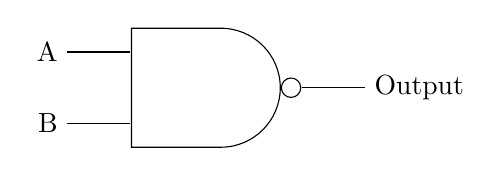
\begin{tikzpicture}[circuit logic US, scale=2]

	\node [nand gate, inputs=nnnn] (nand1) at (0, 0) {};

	\draw (nand1.input 1) -- node[at end, left]{A} ++(left: 4mm);
	\draw (nand1.input 4) -- node[at end, left]{B} ++(left: 4mm);
	\draw (nand1.output) -- node[at end, right]{Output} ++(right: 4mm);

\end{tikzpicture}
\end{center}

\nl
Tablica prawdy (zależności wartości wyjścia bramki od wartości wejść):

{
\centering
\begin{center}
\begin{tabular}{ | c | c | c | } 
  \hline
  \ \ \ \textbf{A} \ \ \ & \ \ \ \textbf{B} \ \ \ & \textbf{Output} \\ 
  \hline
  0 & 0 & 1 \\
  \hline
  0 & 1 & 1 \\
  \hline
  1 & 0 & 1 \\
  \hline
  1 & 1 & 0 \\
  \hline
\end{tabular}
\end{center}
}

\newpage
\paragraph{NOR \\}

Bramka NOR z wejściami \textit{A} i \textit{B} realizuje funkcję NOT-OR, czyli 

$$ NOT \ ( \ \textit{A} \ OR \ \textit{B} \ ) $$

\nl
Oznaczenie bramki NOR w schematach układów logicznych:
\begin{center}
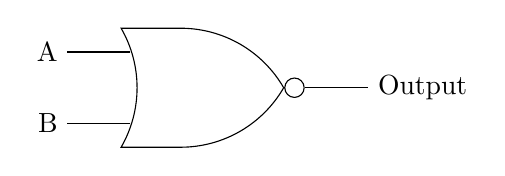
\begin{tikzpicture}[circuit logic US, scale=2]

	\node [nor gate, inputs=nnnn] (nor1) at (0, 0) {};

	\draw (nor1.input 1) -- node[at end, left]{A} ++(left: 4mm);
	\draw (nor1.input 4) -- node[at end, left]{B} ++(left: 4mm);
	\draw (nor1.output) -- node[at end, right]{Output} ++(right: 4mm);

\end{tikzpicture}
\end{center}

\nl
Tablica prawdy:

{
\centering
\begin{center}
\begin{tabular}{ | c | c | c | } 
  \hline
  \ \ \ \textbf{A} \ \ \ & \ \ \ \textbf{B} \ \ \ & \textbf{Output} \\ 
  \hline
  0 & 0 & 1 \\
  \hline
  0 & 1 & 0 \\
  \hline
  1 & 0 & 0 \\
  \hline
  1 & 1 & 0 \\
  \hline
\end{tabular}
\end{center}
}

\nl
\paragraph{XOR \\}

Bramka XOR (lub EXOR z wejściami \textit{A} i \textit{B} realizuje funkcję EXCLUSIVE-OR, czyli 

$$ ( \ \textit{A} \ OR \ \textit{B} \ ) \ AND \ ( \ NOT \ ( \ \textit{A} \ AND \ \textit{B} \ ) \ ) $$

\nl
Oznaczenie bramki XOR w schematach układów logicznych:
\begin{center}
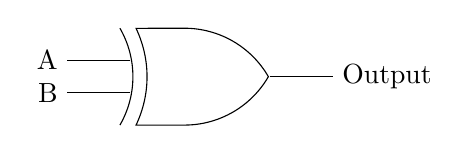
\begin{tikzpicture}[circuit logic US, scale=2]

	\node [xor gate] (xor1) at (0, 0) {};

	\draw (xor1.input 1) -- node[at end, left]{A} ++(left: 4mm);
	\draw (xor1.input 2) -- node[at end, left]{B} ++(left: 4mm);
	\draw (xor1.output) -- node[at end, right]{Output} ++(right: 4mm);

\end{tikzpicture}
\end{center}

\nl
Tablica prawdy:

{
\centering
\begin{center}
\begin{tabular}{ | c | c | c | } 
  \hline
  \ \ \ \textbf{A} \ \ \ & \ \ \ \textbf{B} \ \ \ & \textbf{Output} \\ 
  \hline
  0 & 0 & 0 \\
  \hline
  0 & 1 & 1 \\
  \hline
  1 & 0 & 1 \\
  \hline
  1 & 1 & 0 \\
  \hline
\end{tabular}
\end{center}
}

\newpage
Elektronicznie bramki logiczne realizowane są za pomocą tranzystorów (elementów elektronicznych mogących pełnić rolę przełącznika sterowanego napięciem). Z historycznego punktu widzenia to właśnie użycie półprzewodników do budowy tranzystorów najmocniej pchnęło do przodu rozwój komputerów. Wcześniej układy logiczne budowano przy użyciu lamp próżniowych. Użycie tranzystorów półprzewodnikowych pozwoliło zmniejszyć rozmiary i efektywność bramek logicznych, a co za tym idzie procesorów i układów pamięci. Dla przykładu poniżej zamieszczam schemat bramki NAND realizowanej przy pomocy tranzystorów typu NPN: \\

\begin{center}
\begin{circuitikz}[scale=1.2]

  	\draw (0,0) node[npn] (npn1) {};
	\draw ($(npn1)-(0.1,0)$) circle [radius=18pt];

	\draw (0,-3) node[npn] (npn2) {};
	\draw ($(npn2)-(0.1,0)$) circle [radius=18pt];

	\draw (npn1.emitter) to (npn2.collector);

	\draw (npn2.emitter) to (0,-5) node[ground]{};

	\draw (npn1.collector) to (0,1)
				to [R=$R_1$] (0,4.5)
				to (0,4.6) node[vcc]{$V_{cc}$};

	\draw (0,1) to [short,-o] (4, 1) node[anchor=south]{Y};

	\draw (npn1.base) to (-1,0)
				to [R=$R_2$] (-4,0)
				to [short,-o] (-5,0) node[anchor=south]{A};

	\draw (npn2.base) to (-1,-3)
				to [R=$R_2$] (-4,-3)
				to [short,-o] (-5,-3) node[anchor=south]{B};

\end{circuitikz}
\end{center}

\nl 
Tylko w przypadku, kiedy napięcie będzie podane na obydwa wejścia A i B obydwa tranzystory będą "zamknięte", pozwalając napięciu z zasilania ($V_{cc}$) płynąć prosto do masy. W innym przypadku napięcie z zasilania jest obserwowane na wyjściu Y.

\newpage
\paragraph{Ćwiczenie 4.1 \\}
Zapoznanie się z płytką UC-2 do badania układów z scalonych TTL.

\begin{figure}[H]
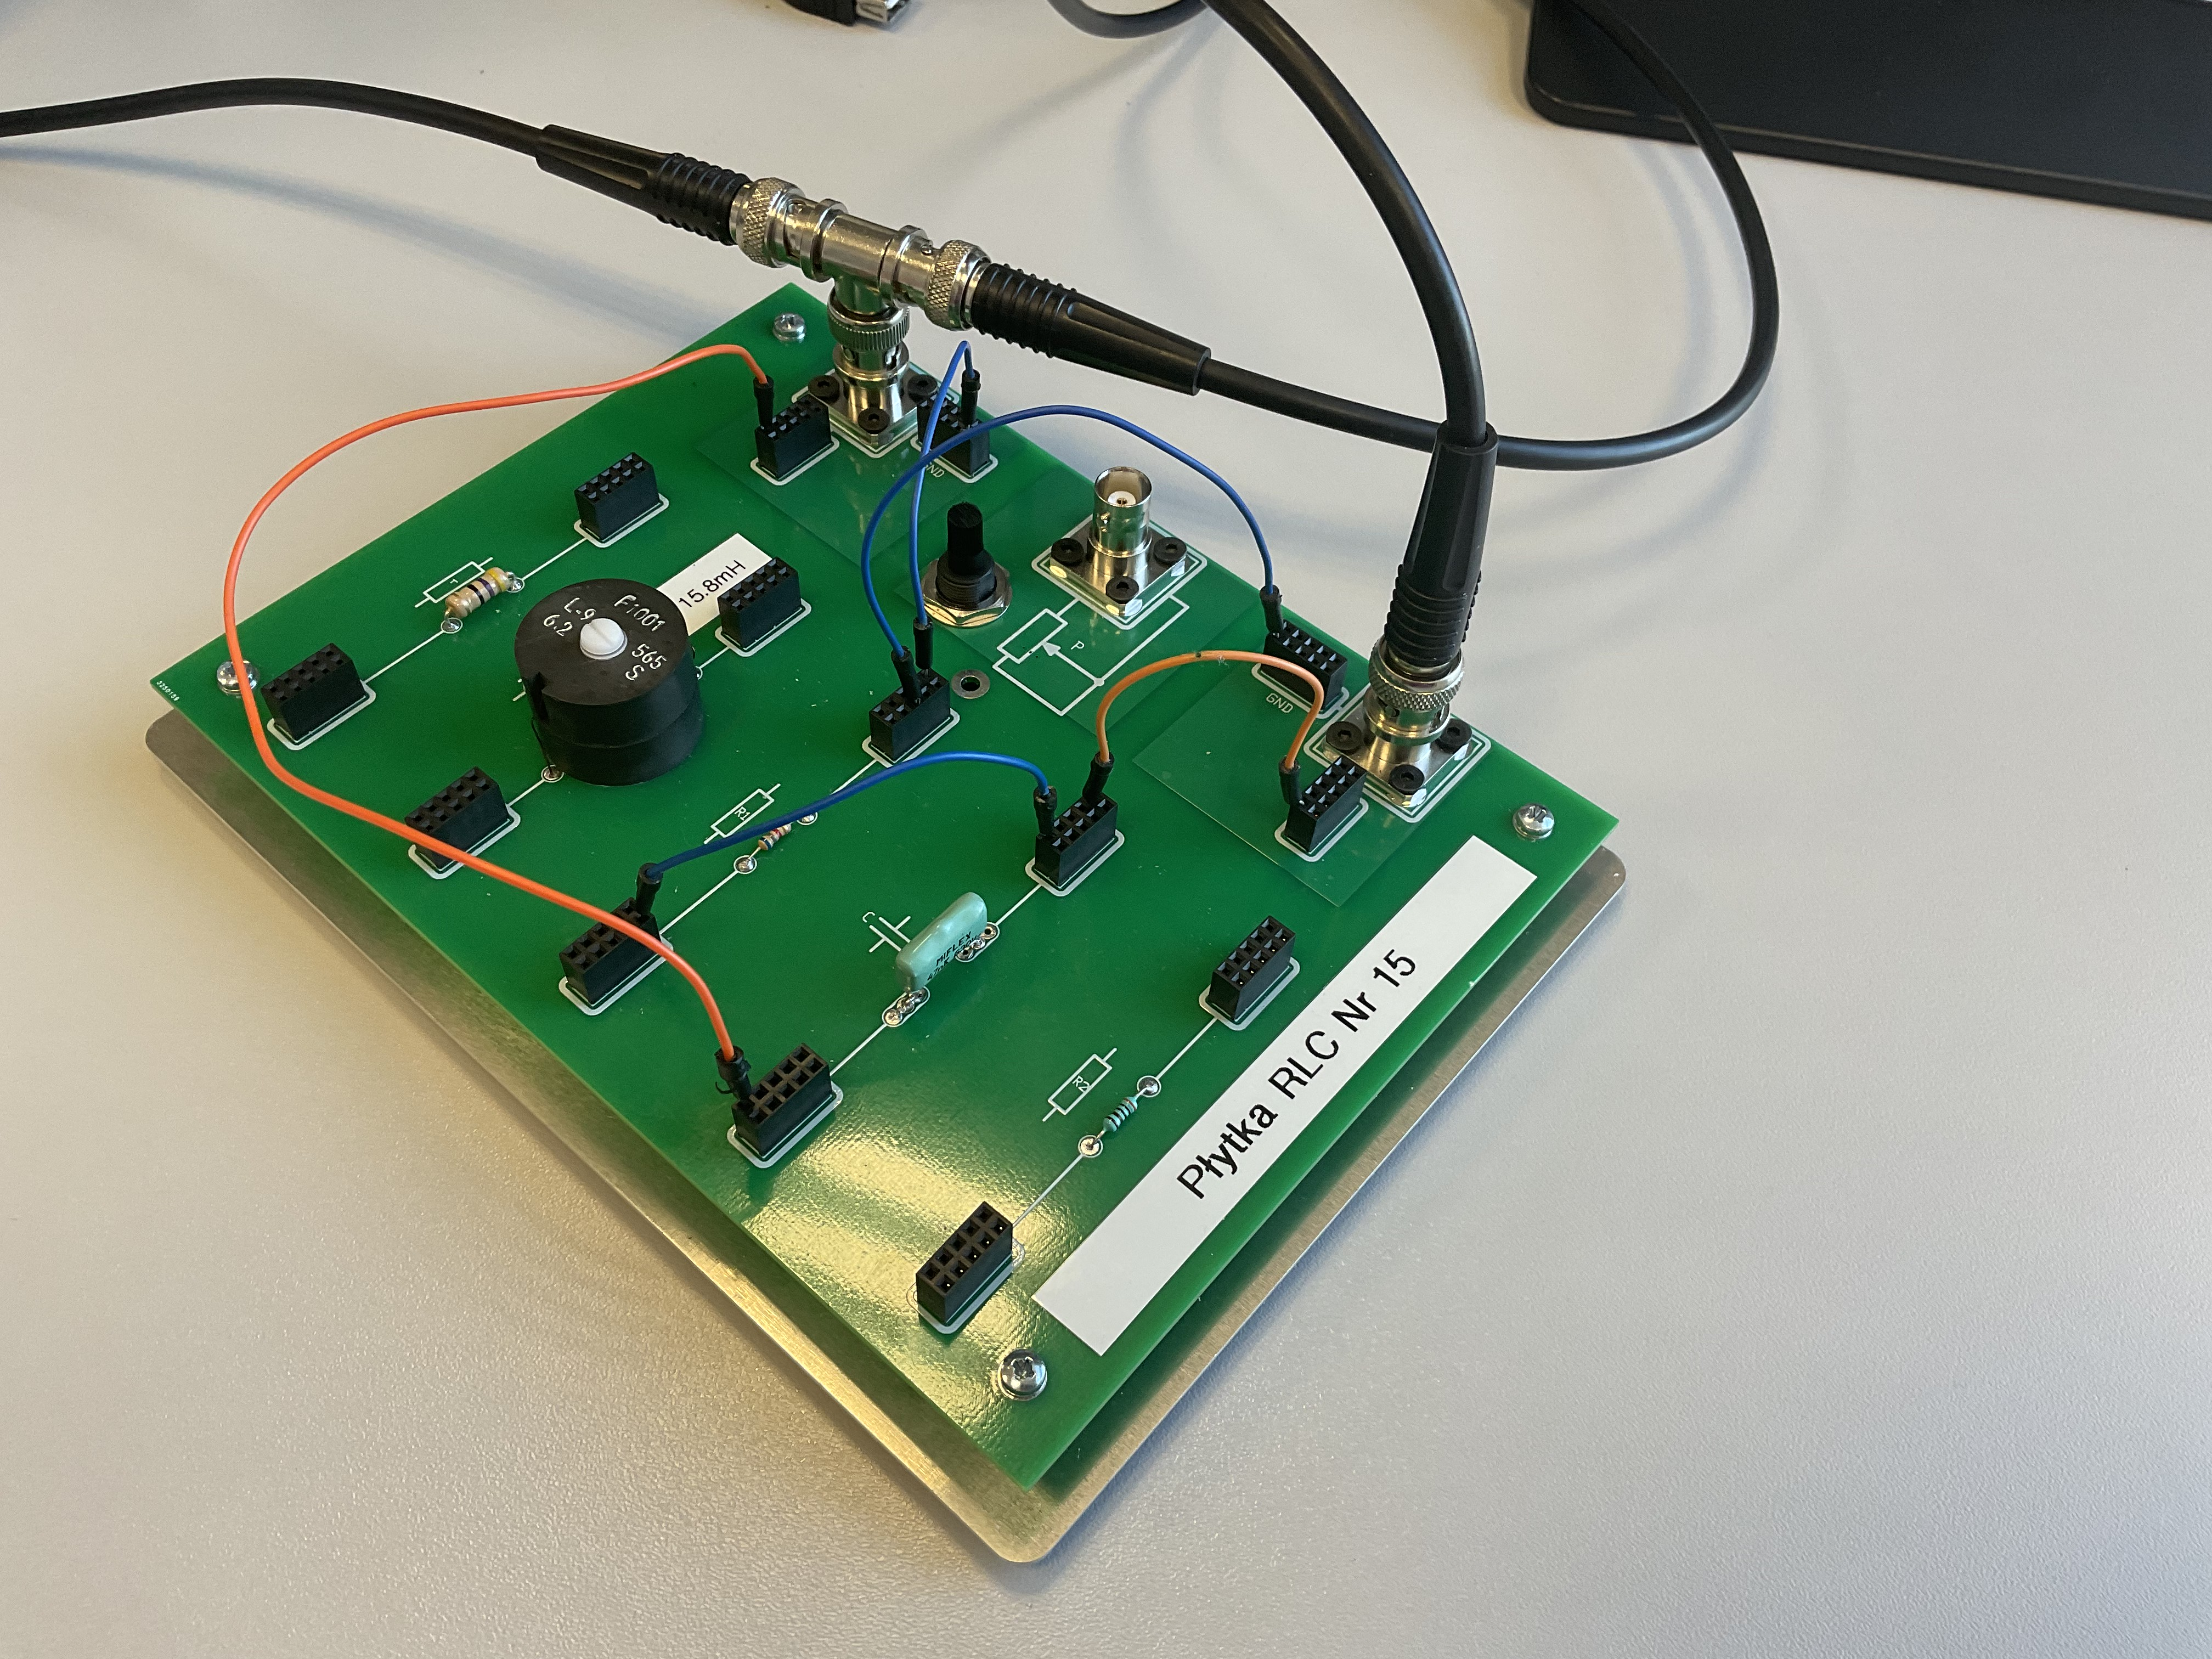
\includegraphics[scale=0.07]{C0}
\centering
\captionsetup{labelformat=empty}
\caption{Płytka UC-2.}
\end{figure}

Na płytce znajdują się dwa impulsatory do wytwarzania sygnałów logicznych, próbnik stanów logicznych (komparator do sprawdzania wartości logicznej sygnału), osiem diod, dwa złącza BNC oraz dwa gniazda na układy scalone: 16-pinowe i 14-pinowe. Obok gniazd znajdują się także piny zasilające ($5 \ V$) oraz masy ($0 \ V$). \\

\newpage
Zmierzyłem napięcia na pinach $5 \ V$ oraz na wyjściach impulsatorów. Każdy impulsator ma wyjście $Q$ oraz wyjście zaprzeczone $\overline{Q}$. Na wyjście $Q$ w stanie domyślnym podane jest $0 \ V$ (logiczny stan fałszu - FALSE), a na wyjście $\overline{Q}$ - $5 \ V$ (logiczny stan prawdy - TRUE). Naciśnięcie przycisku powoduje zamianę stanów - $Q$ na TRUE i $\overline{Q}$ na FALSE.

\begin{figure}[H]
    \centering
    \subfloat[\centering Napięcie $5 \ V$]{{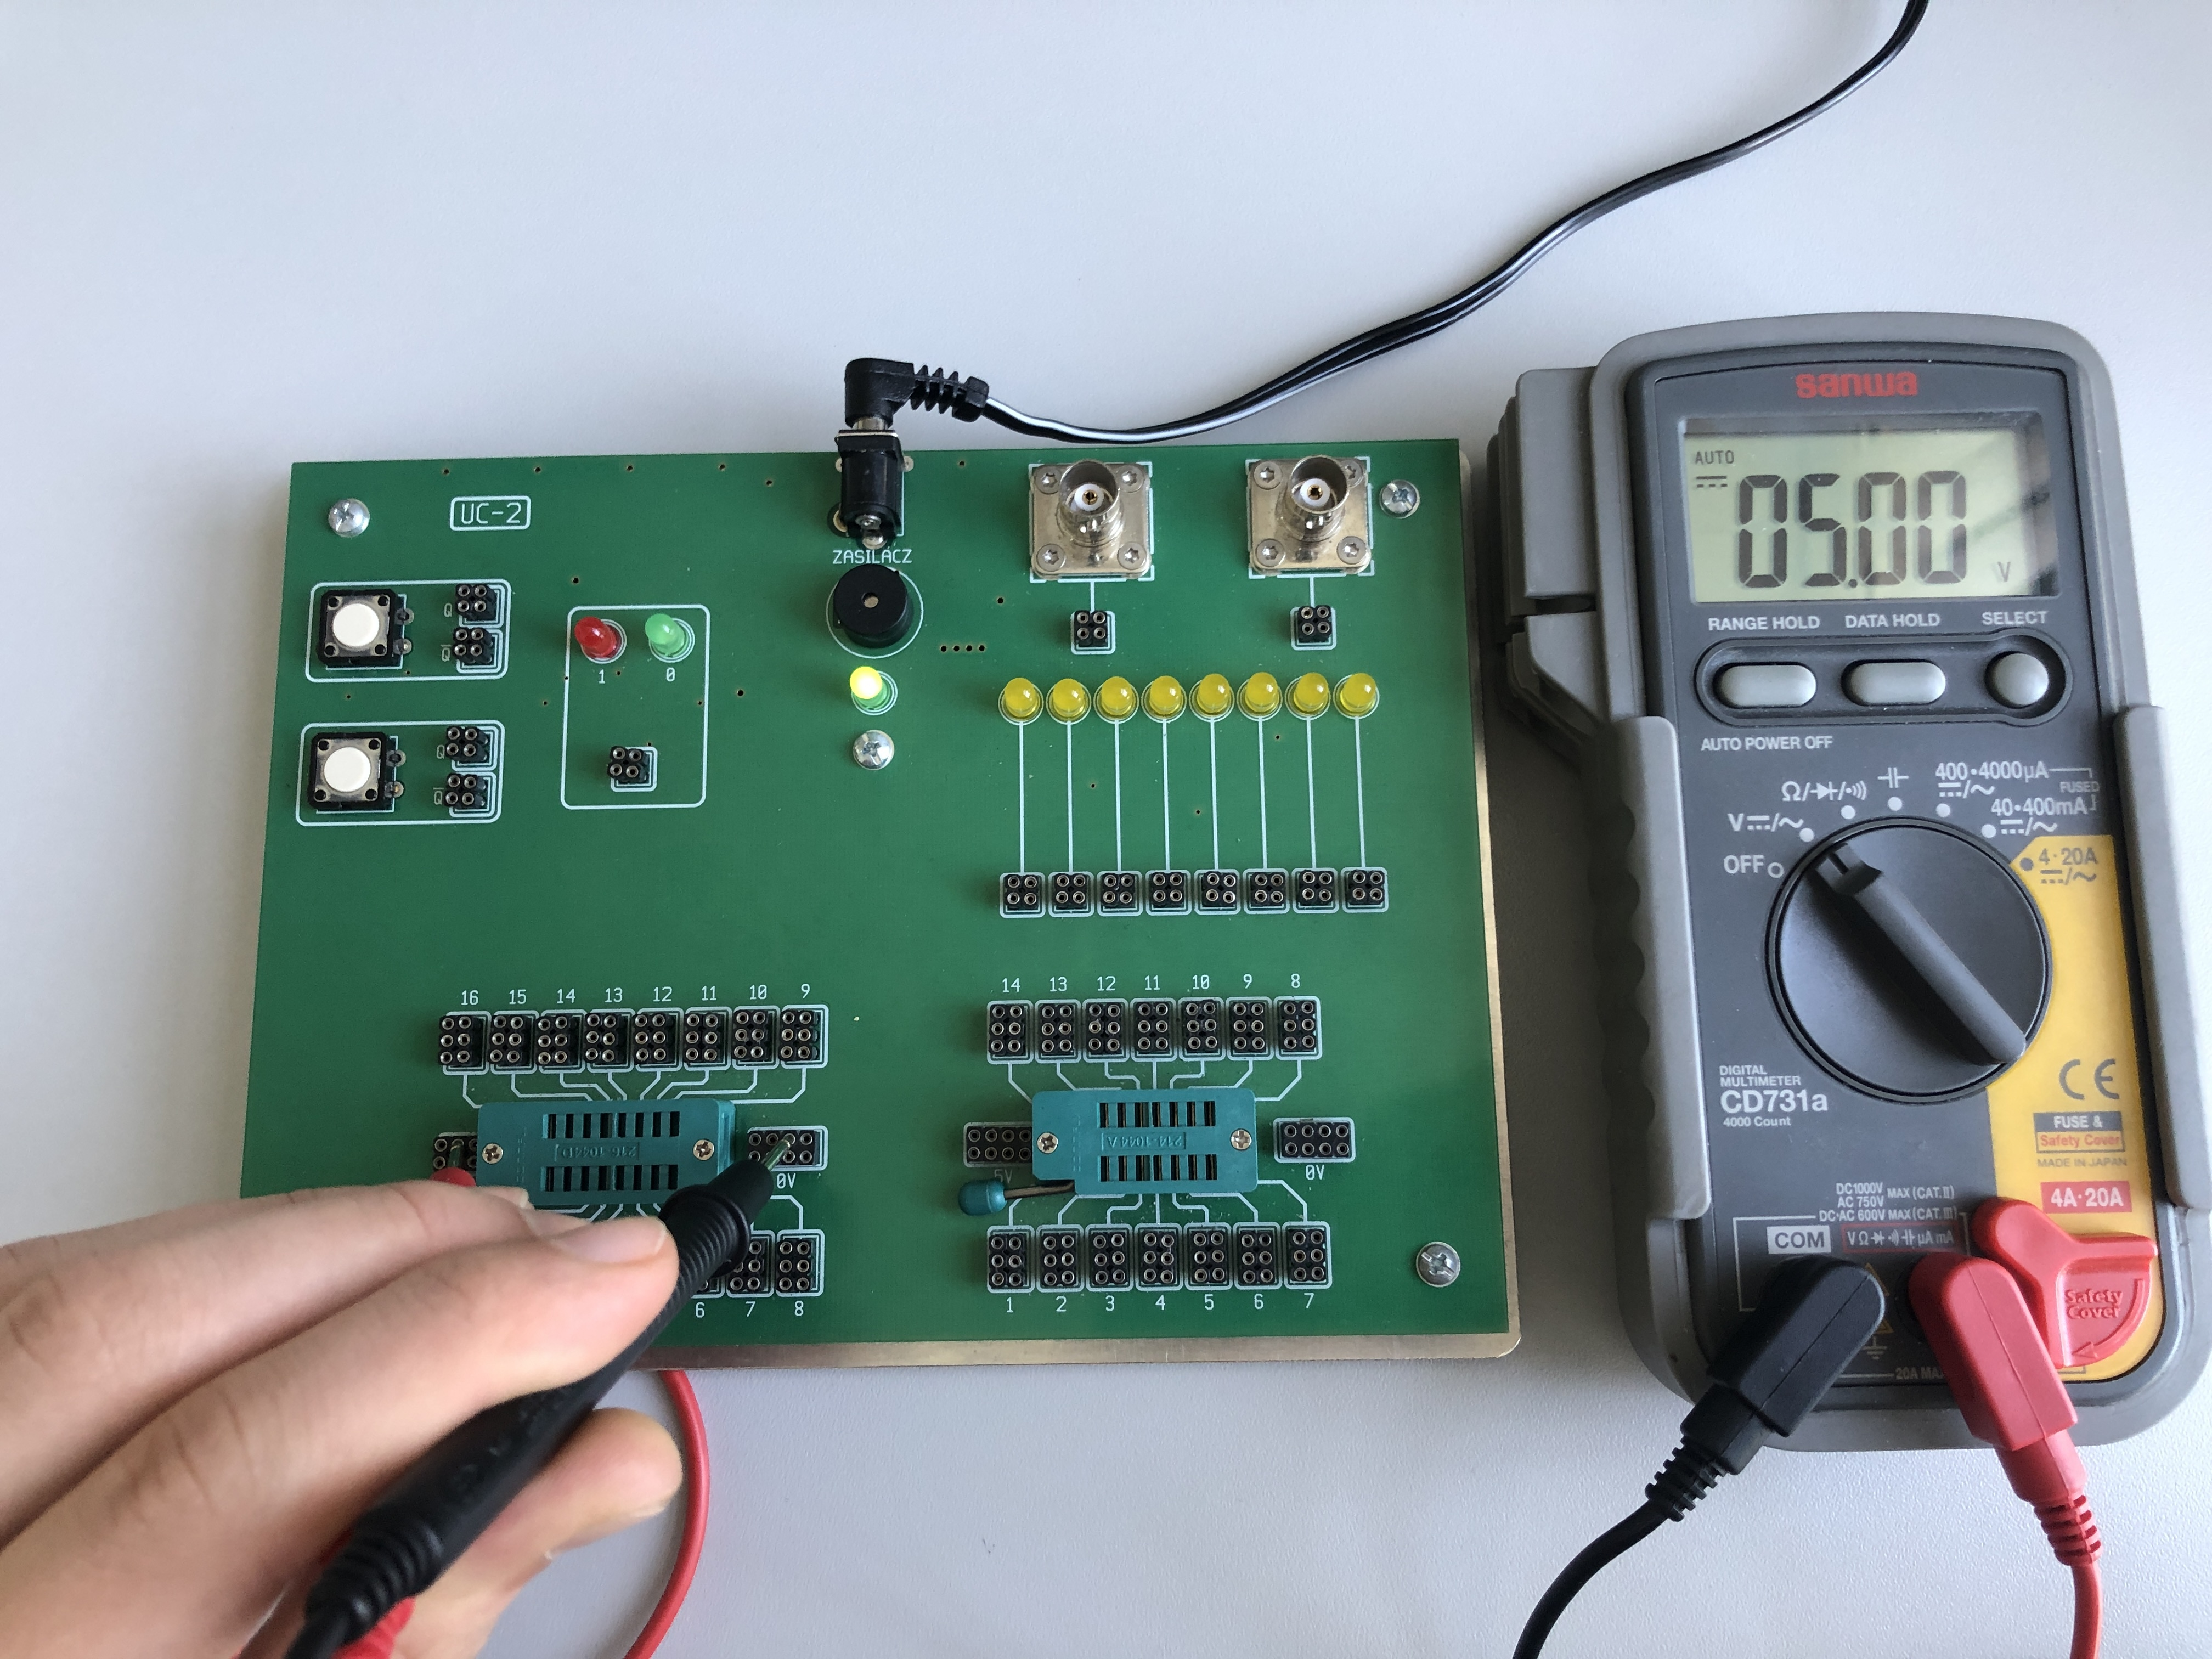
\includegraphics[width=7cm]{C62}}}%
    \qquad
    \subfloat[\centering Napięcie $5 \ V$]{{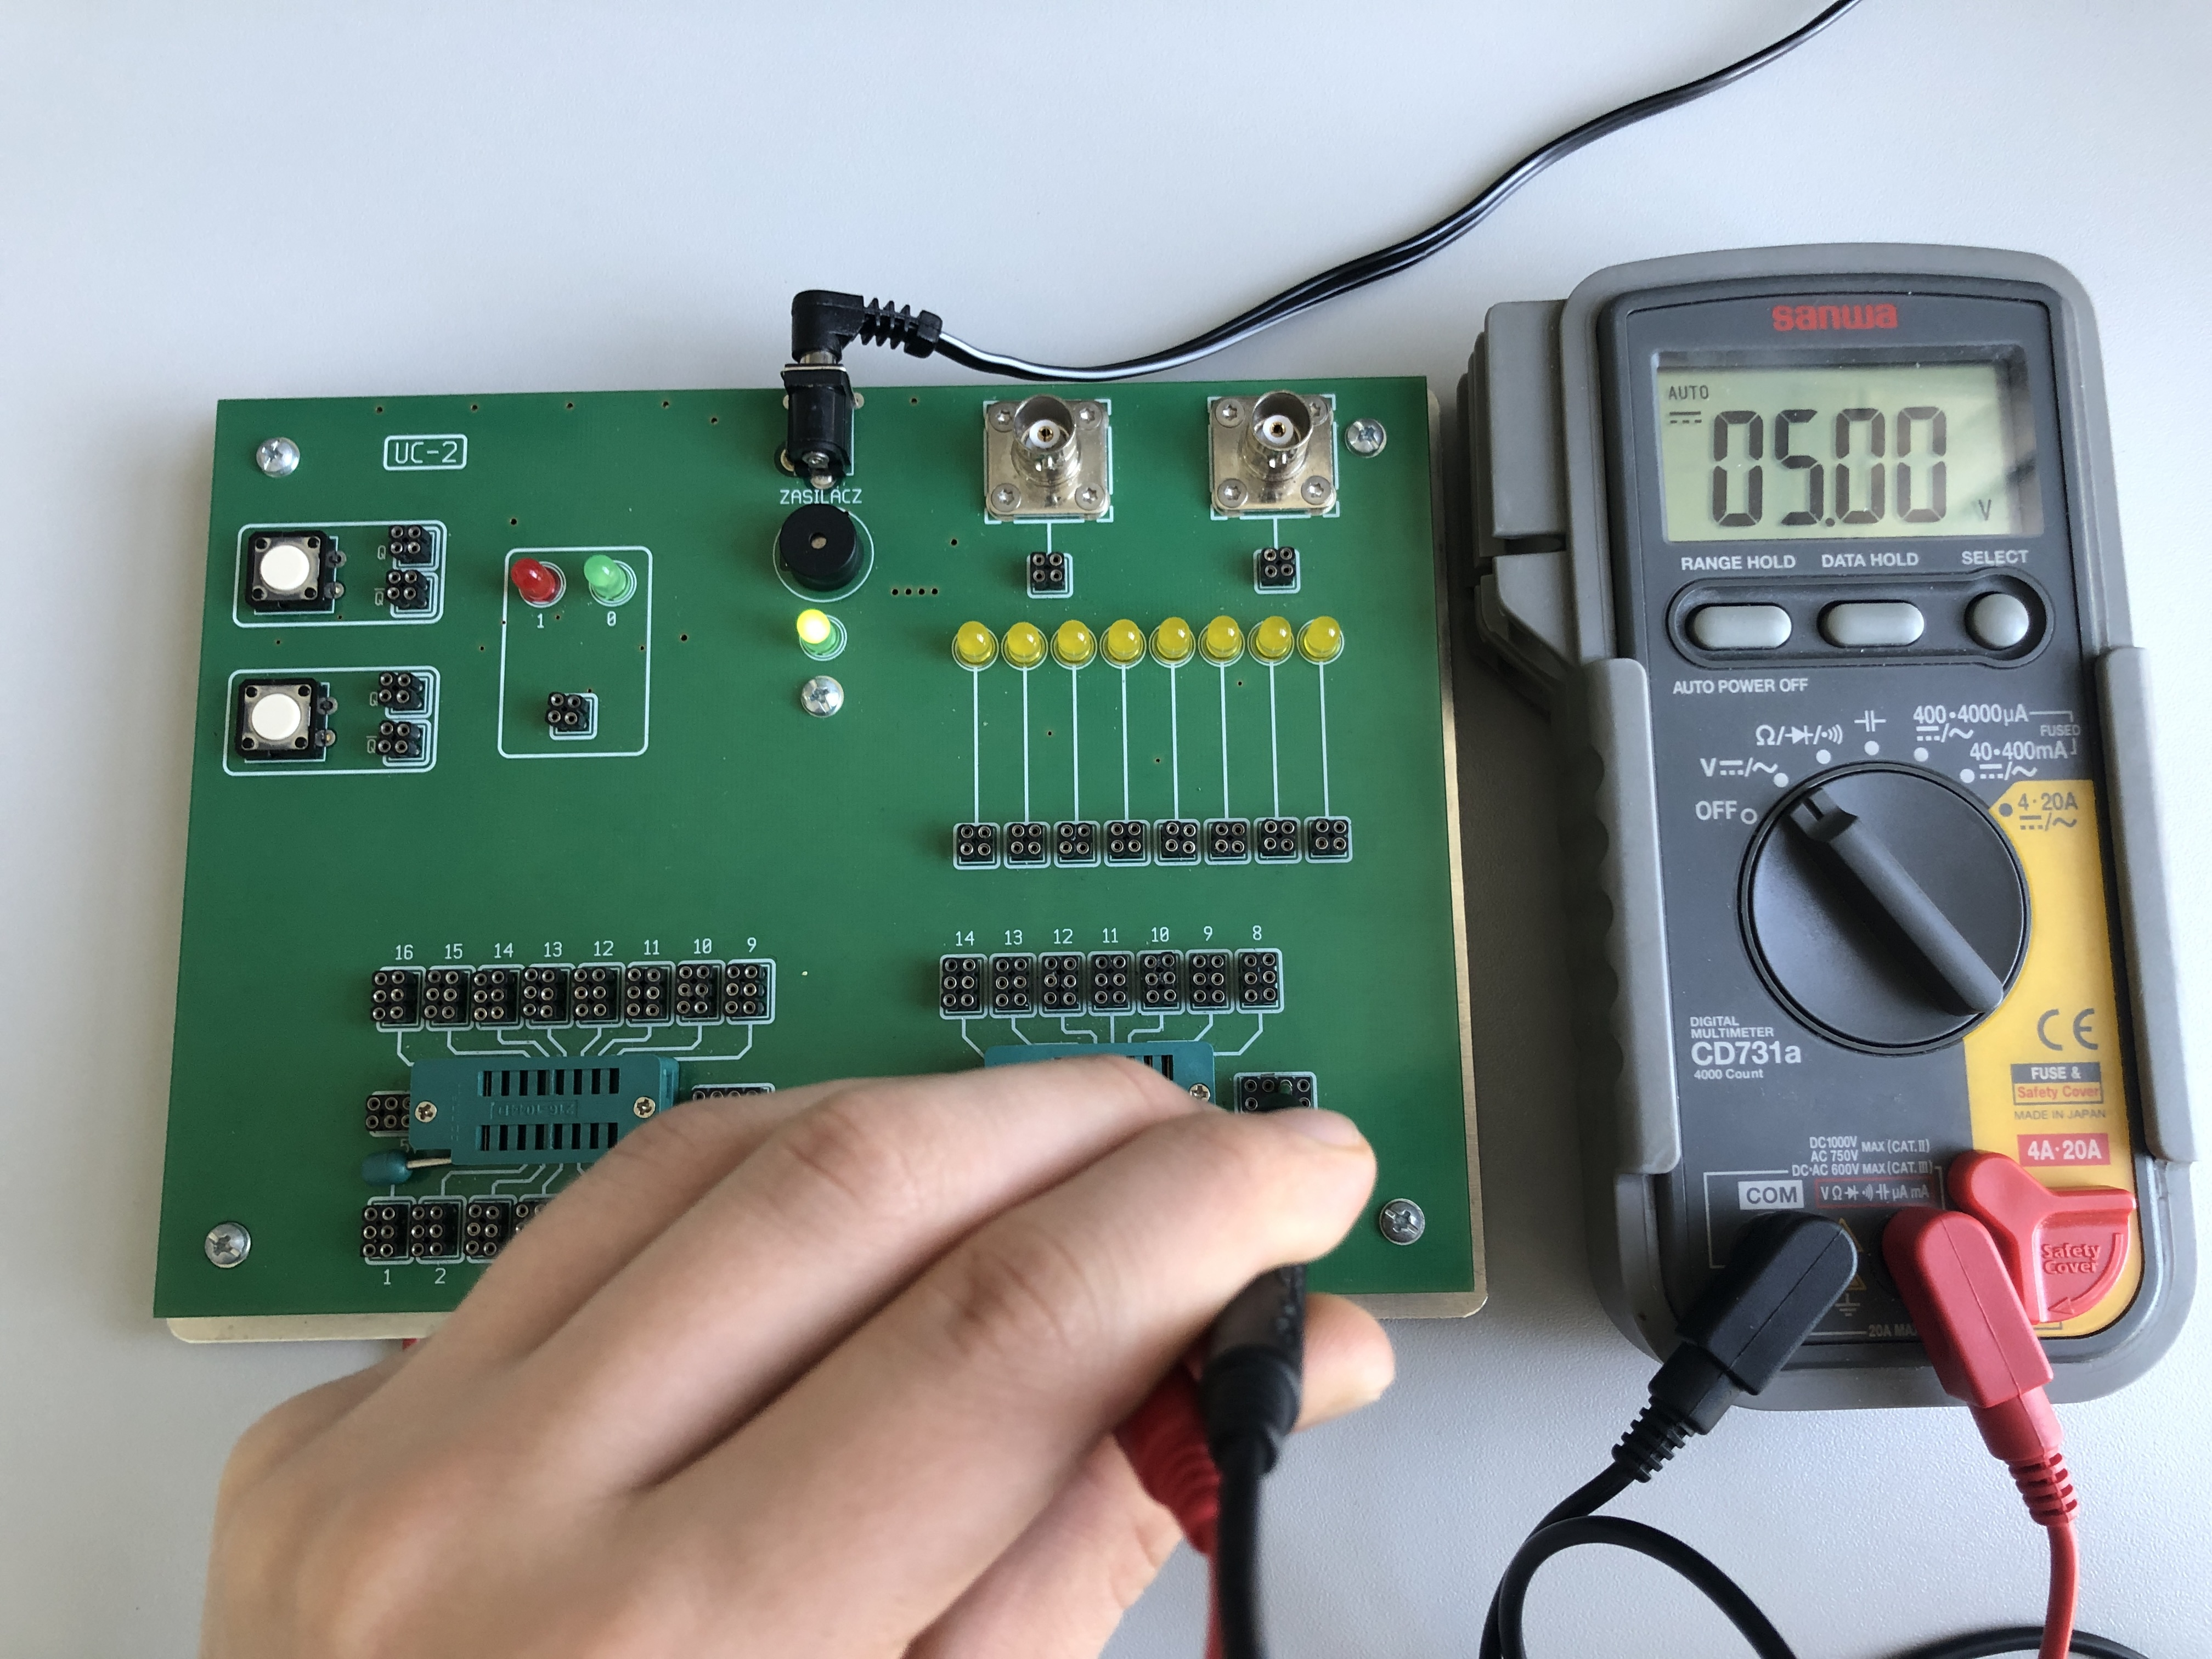
\includegraphics[width=7cm]{C63}}}%
\end{figure}

\begin{figure}[H]
    \centering
    \subfloat[\centering Wyjście $\overline{Q}$ impulsatora]{{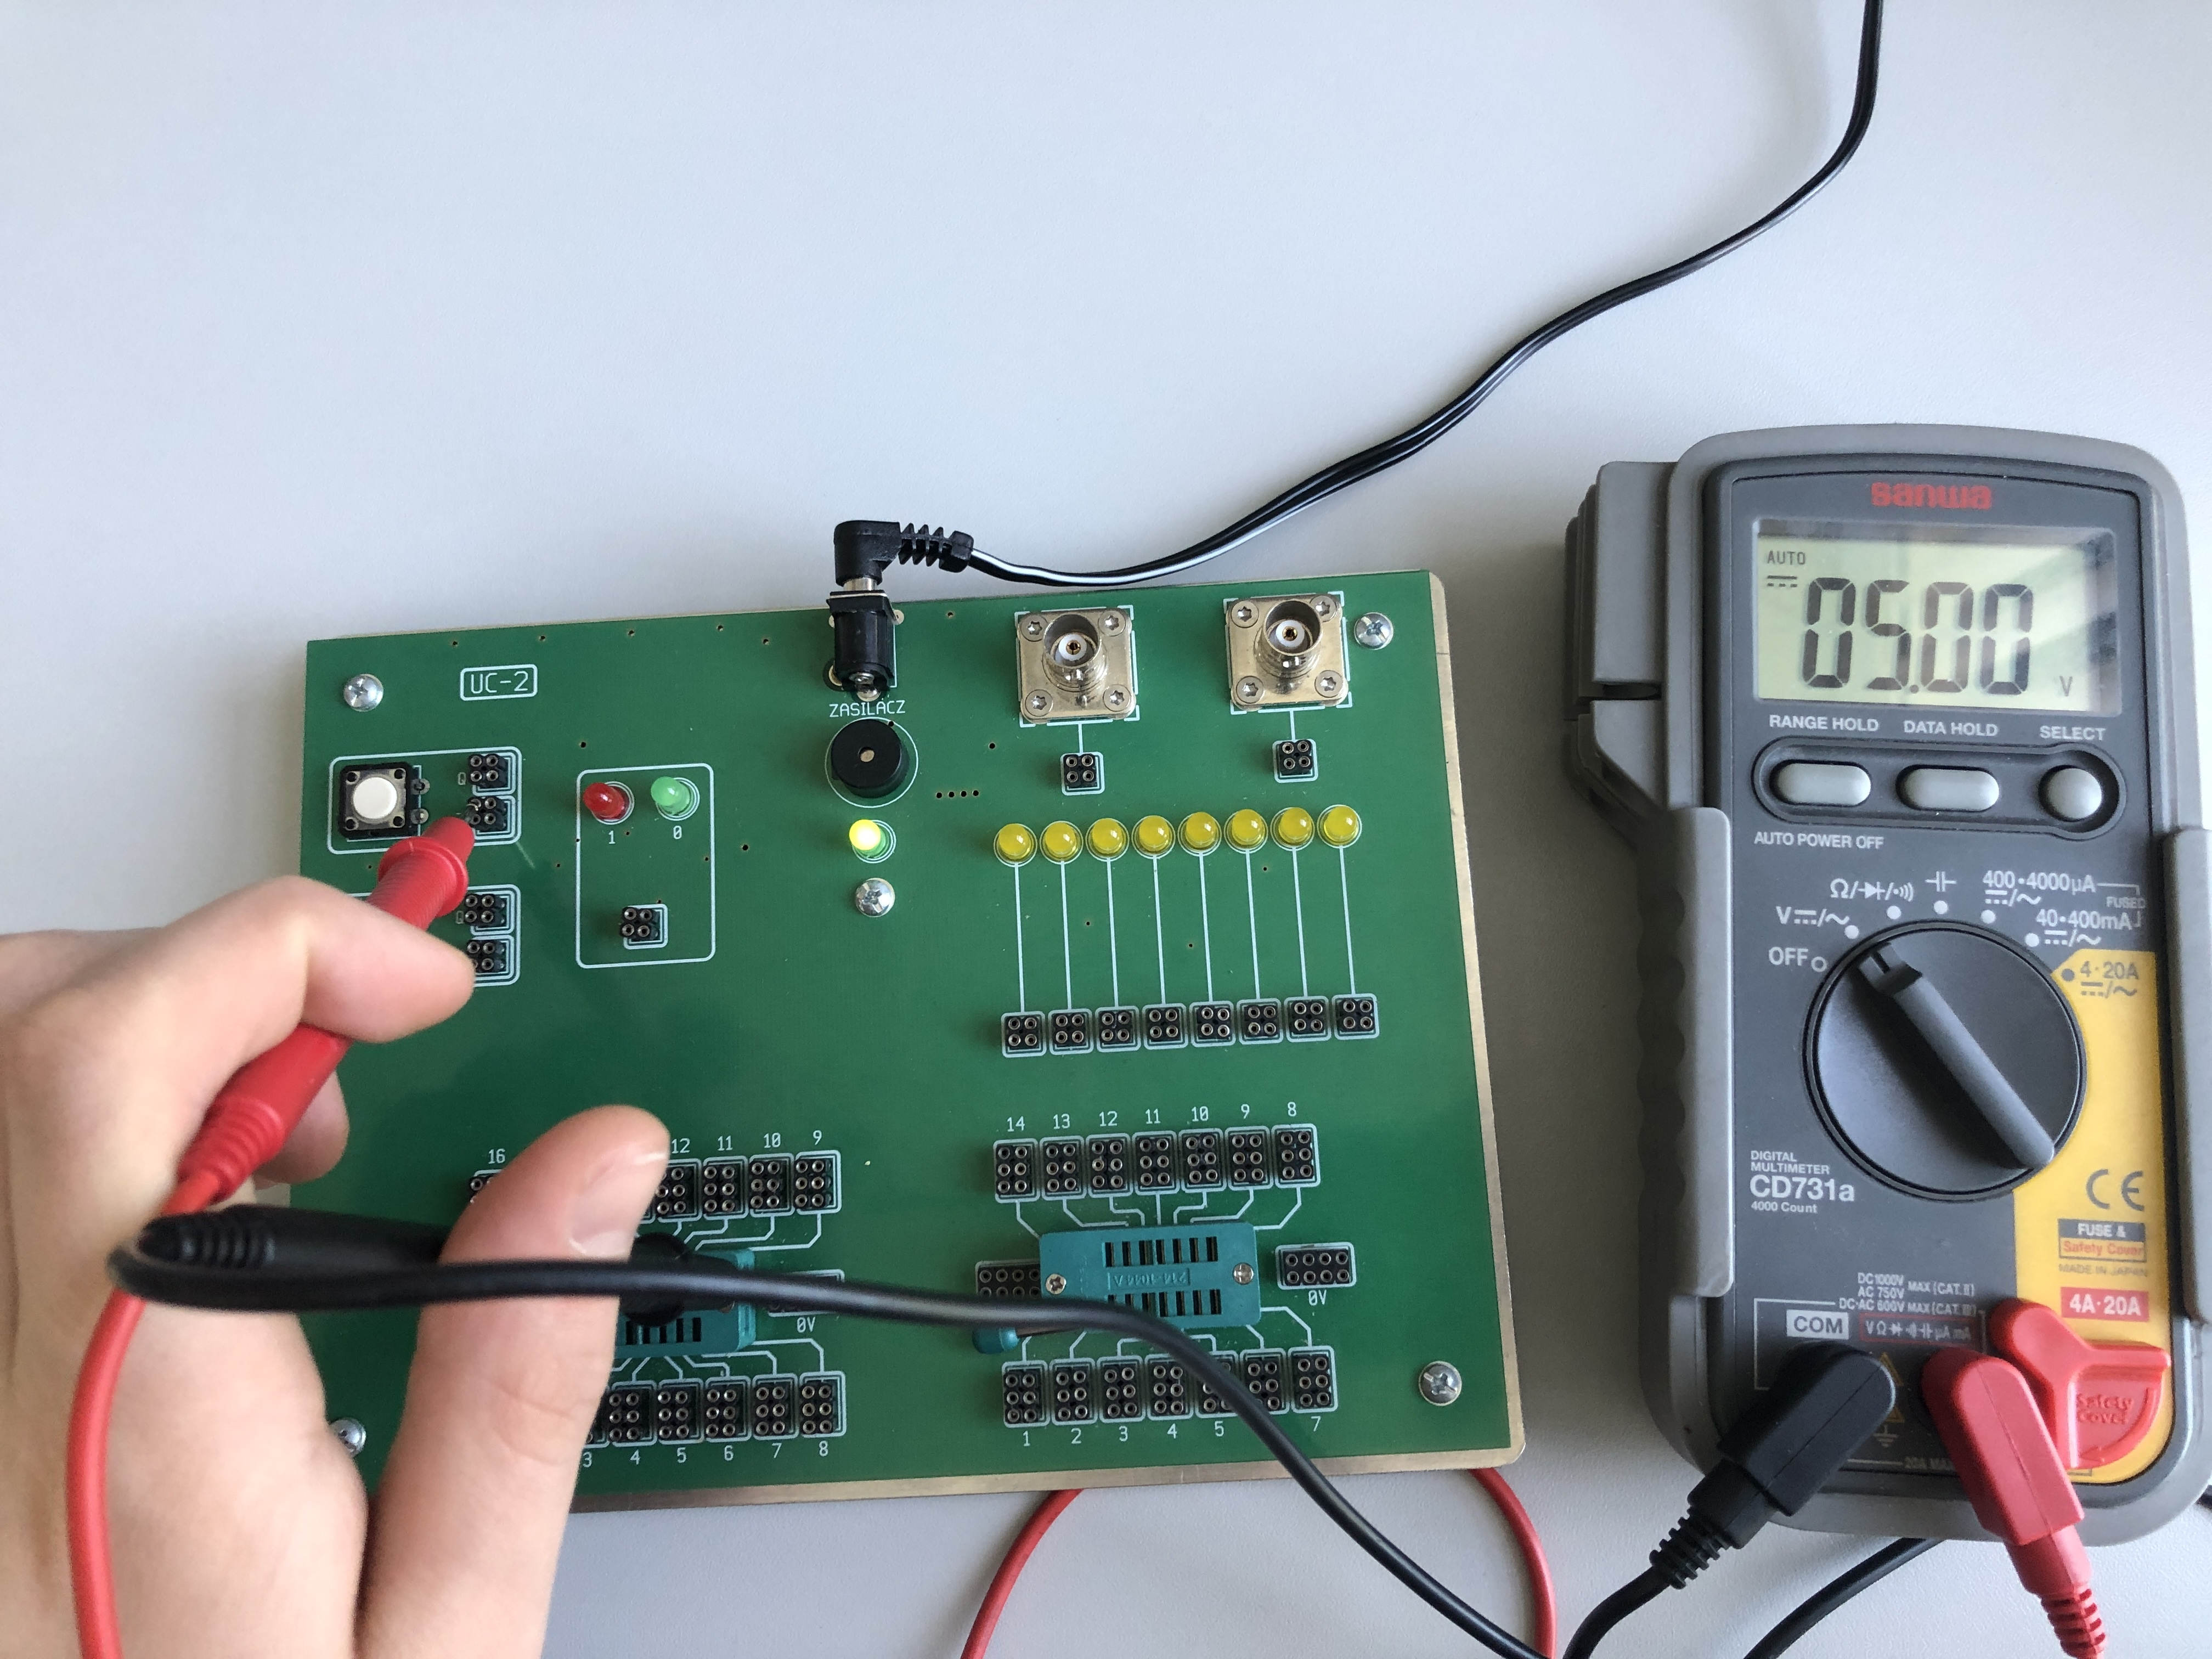
\includegraphics[width=7cm]{C64}}}%
    \qquad
    \subfloat[\centering Wyjście $Q$ impulsatora]{{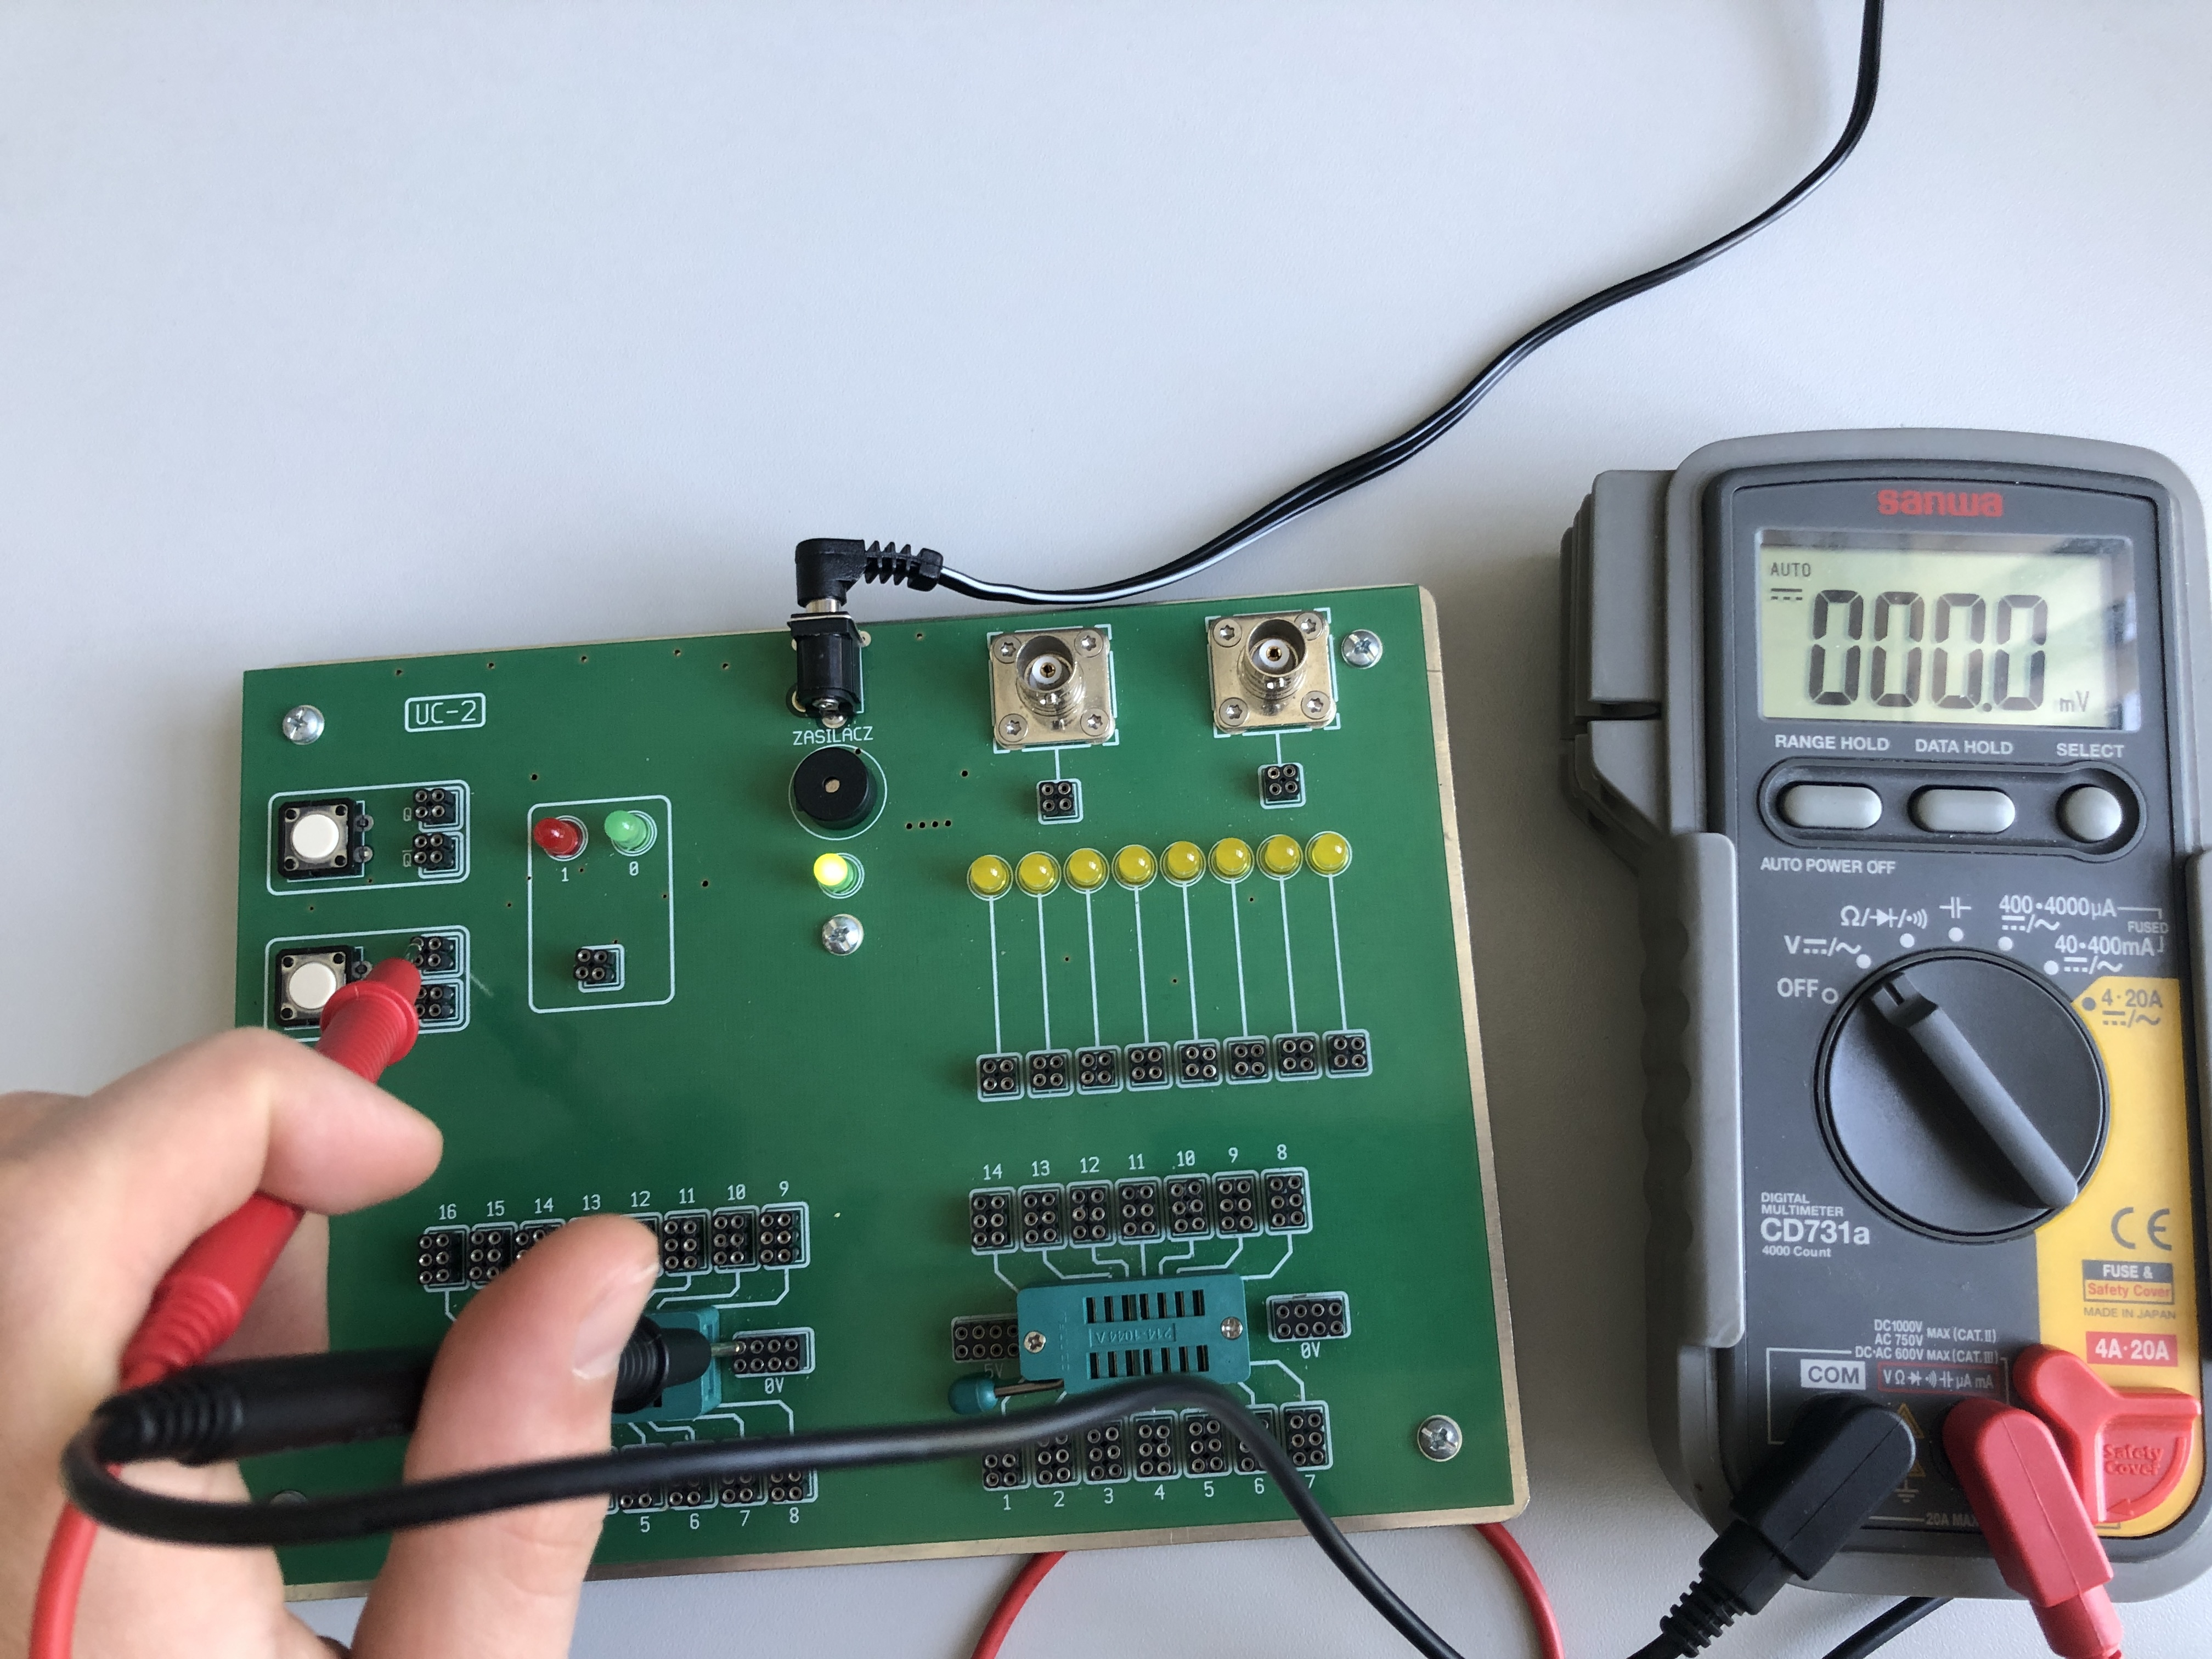
\includegraphics[width=7cm]{C65}}}%
\end{figure}

\begin{figure}[H]
    \centering
    \subfloat[\centering Sygnał logiczny TRUE na wyjściu $Q$ impulsatora]{{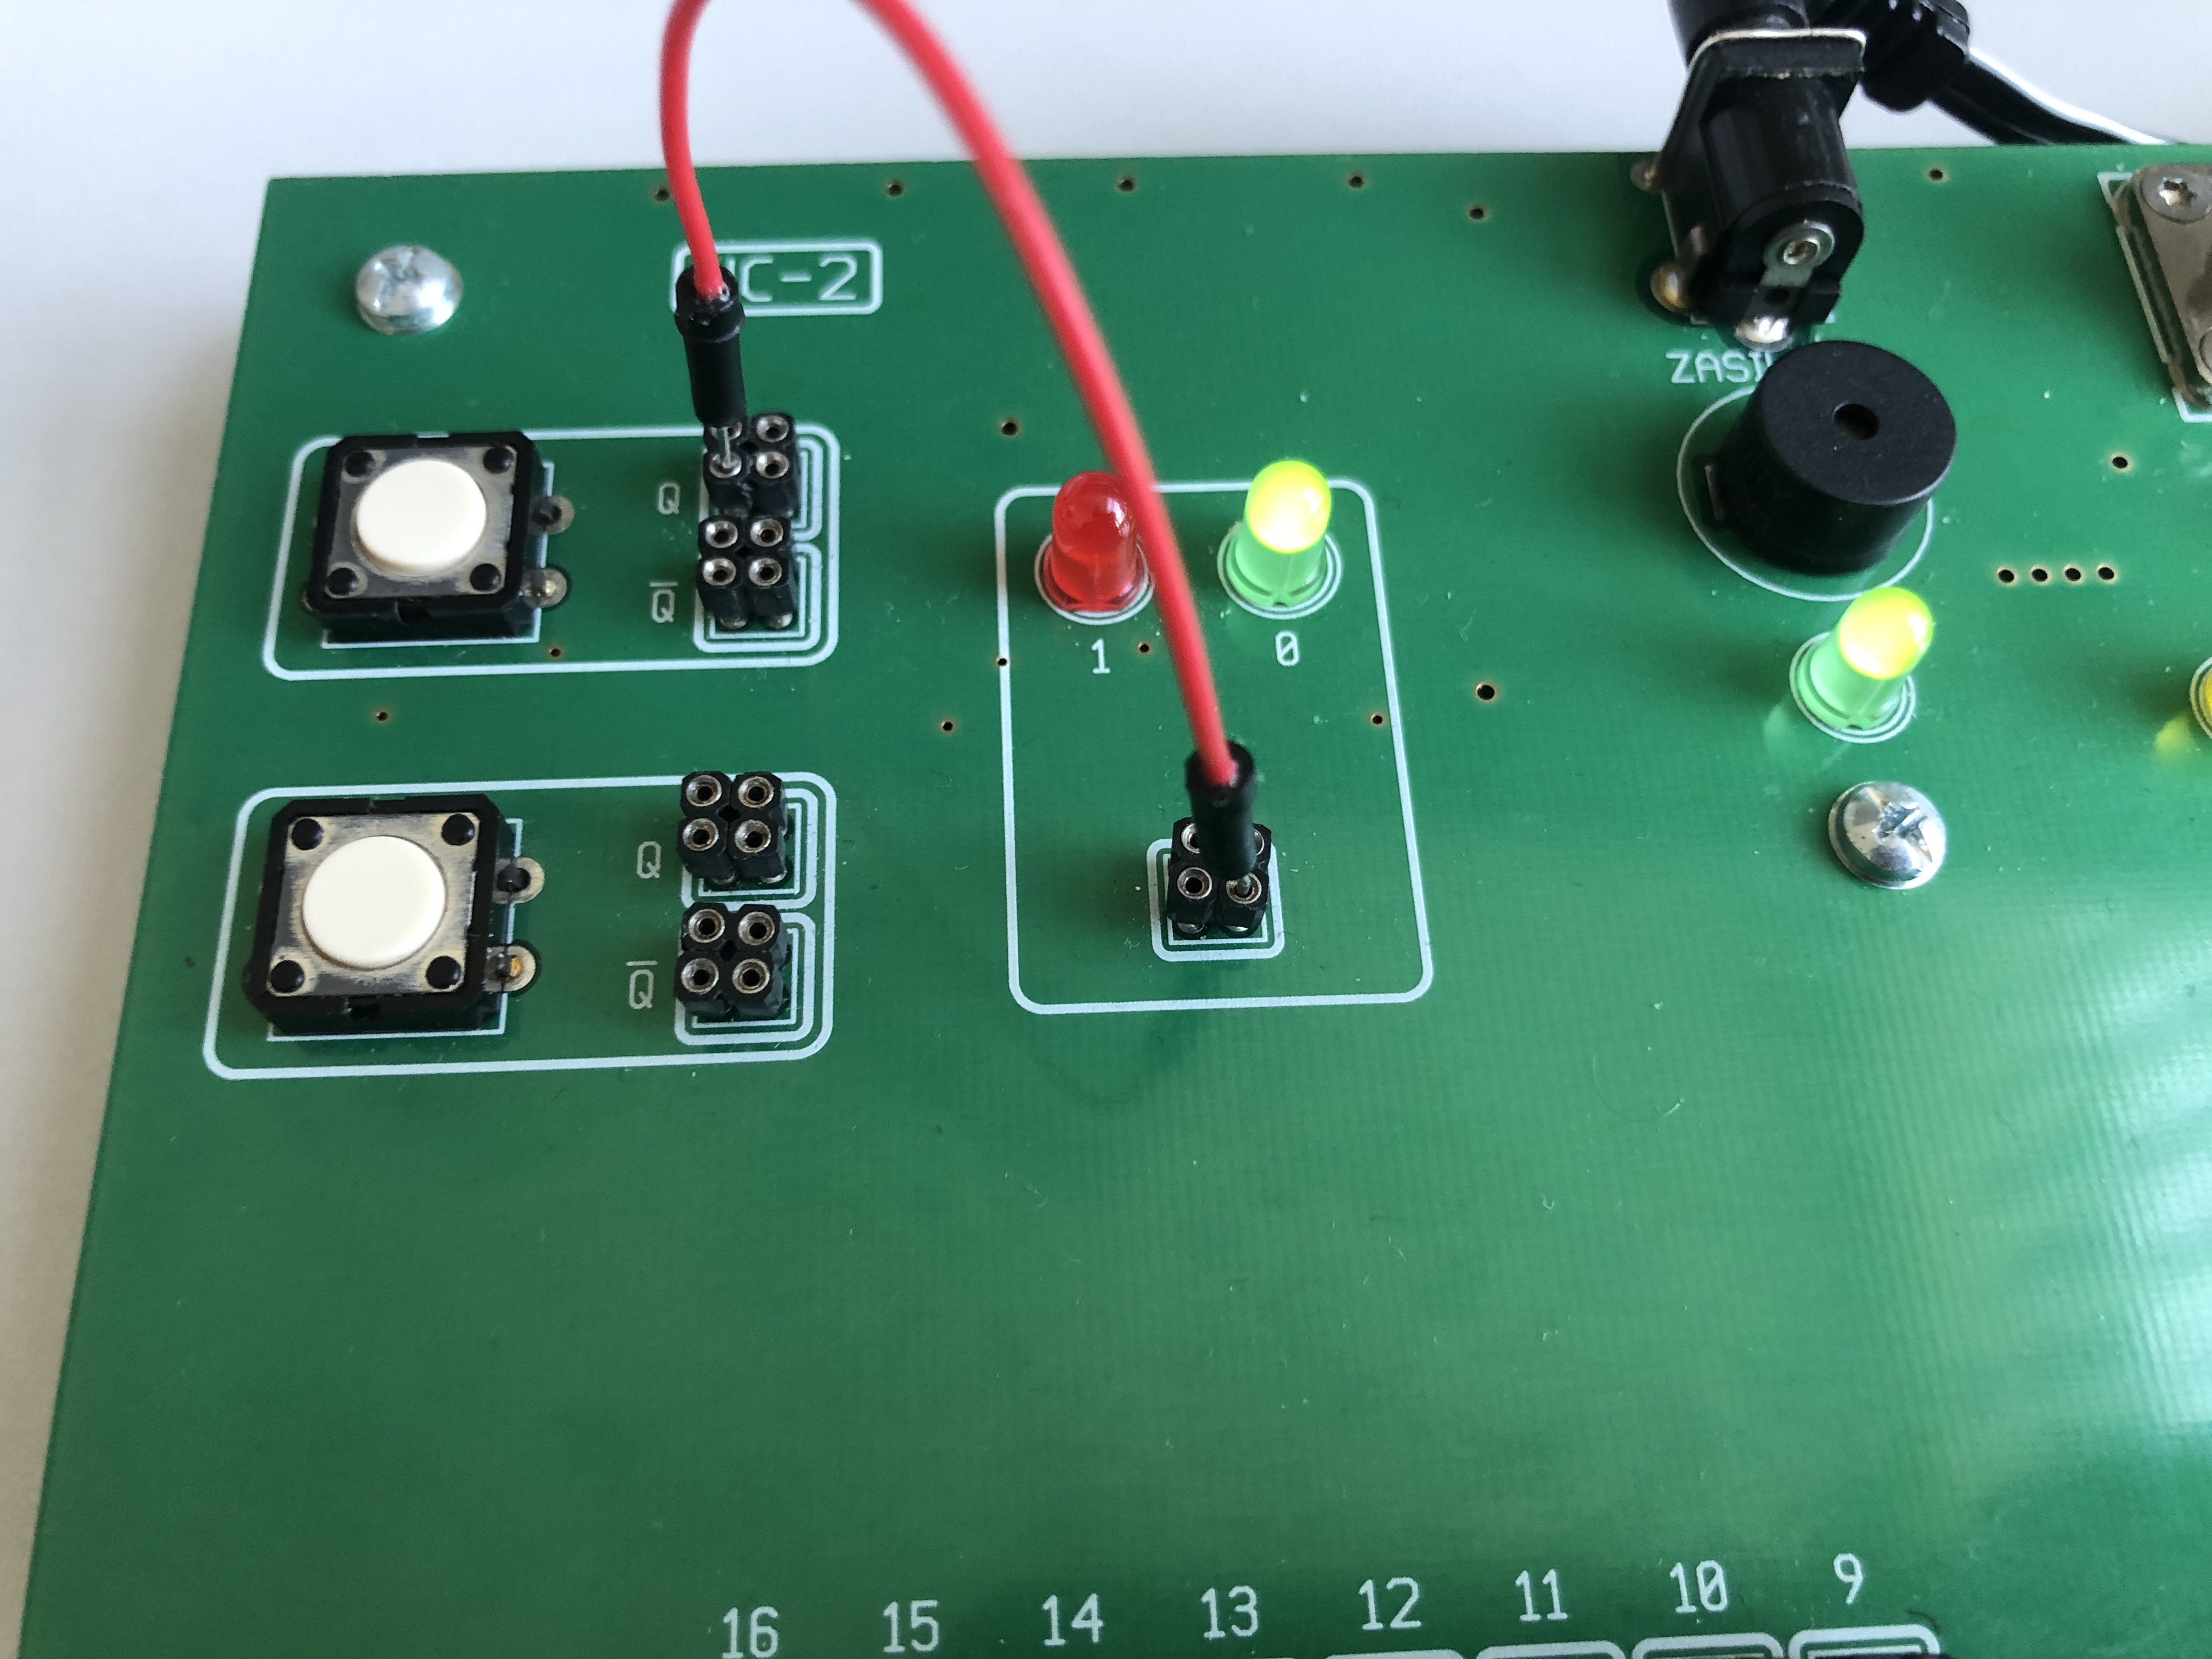
\includegraphics[width=7cm]{C66}}}%
    \qquad
    \subfloat[\centering Sygnał logiczny FALSE na wyjściu $Q$ impulsatora]{{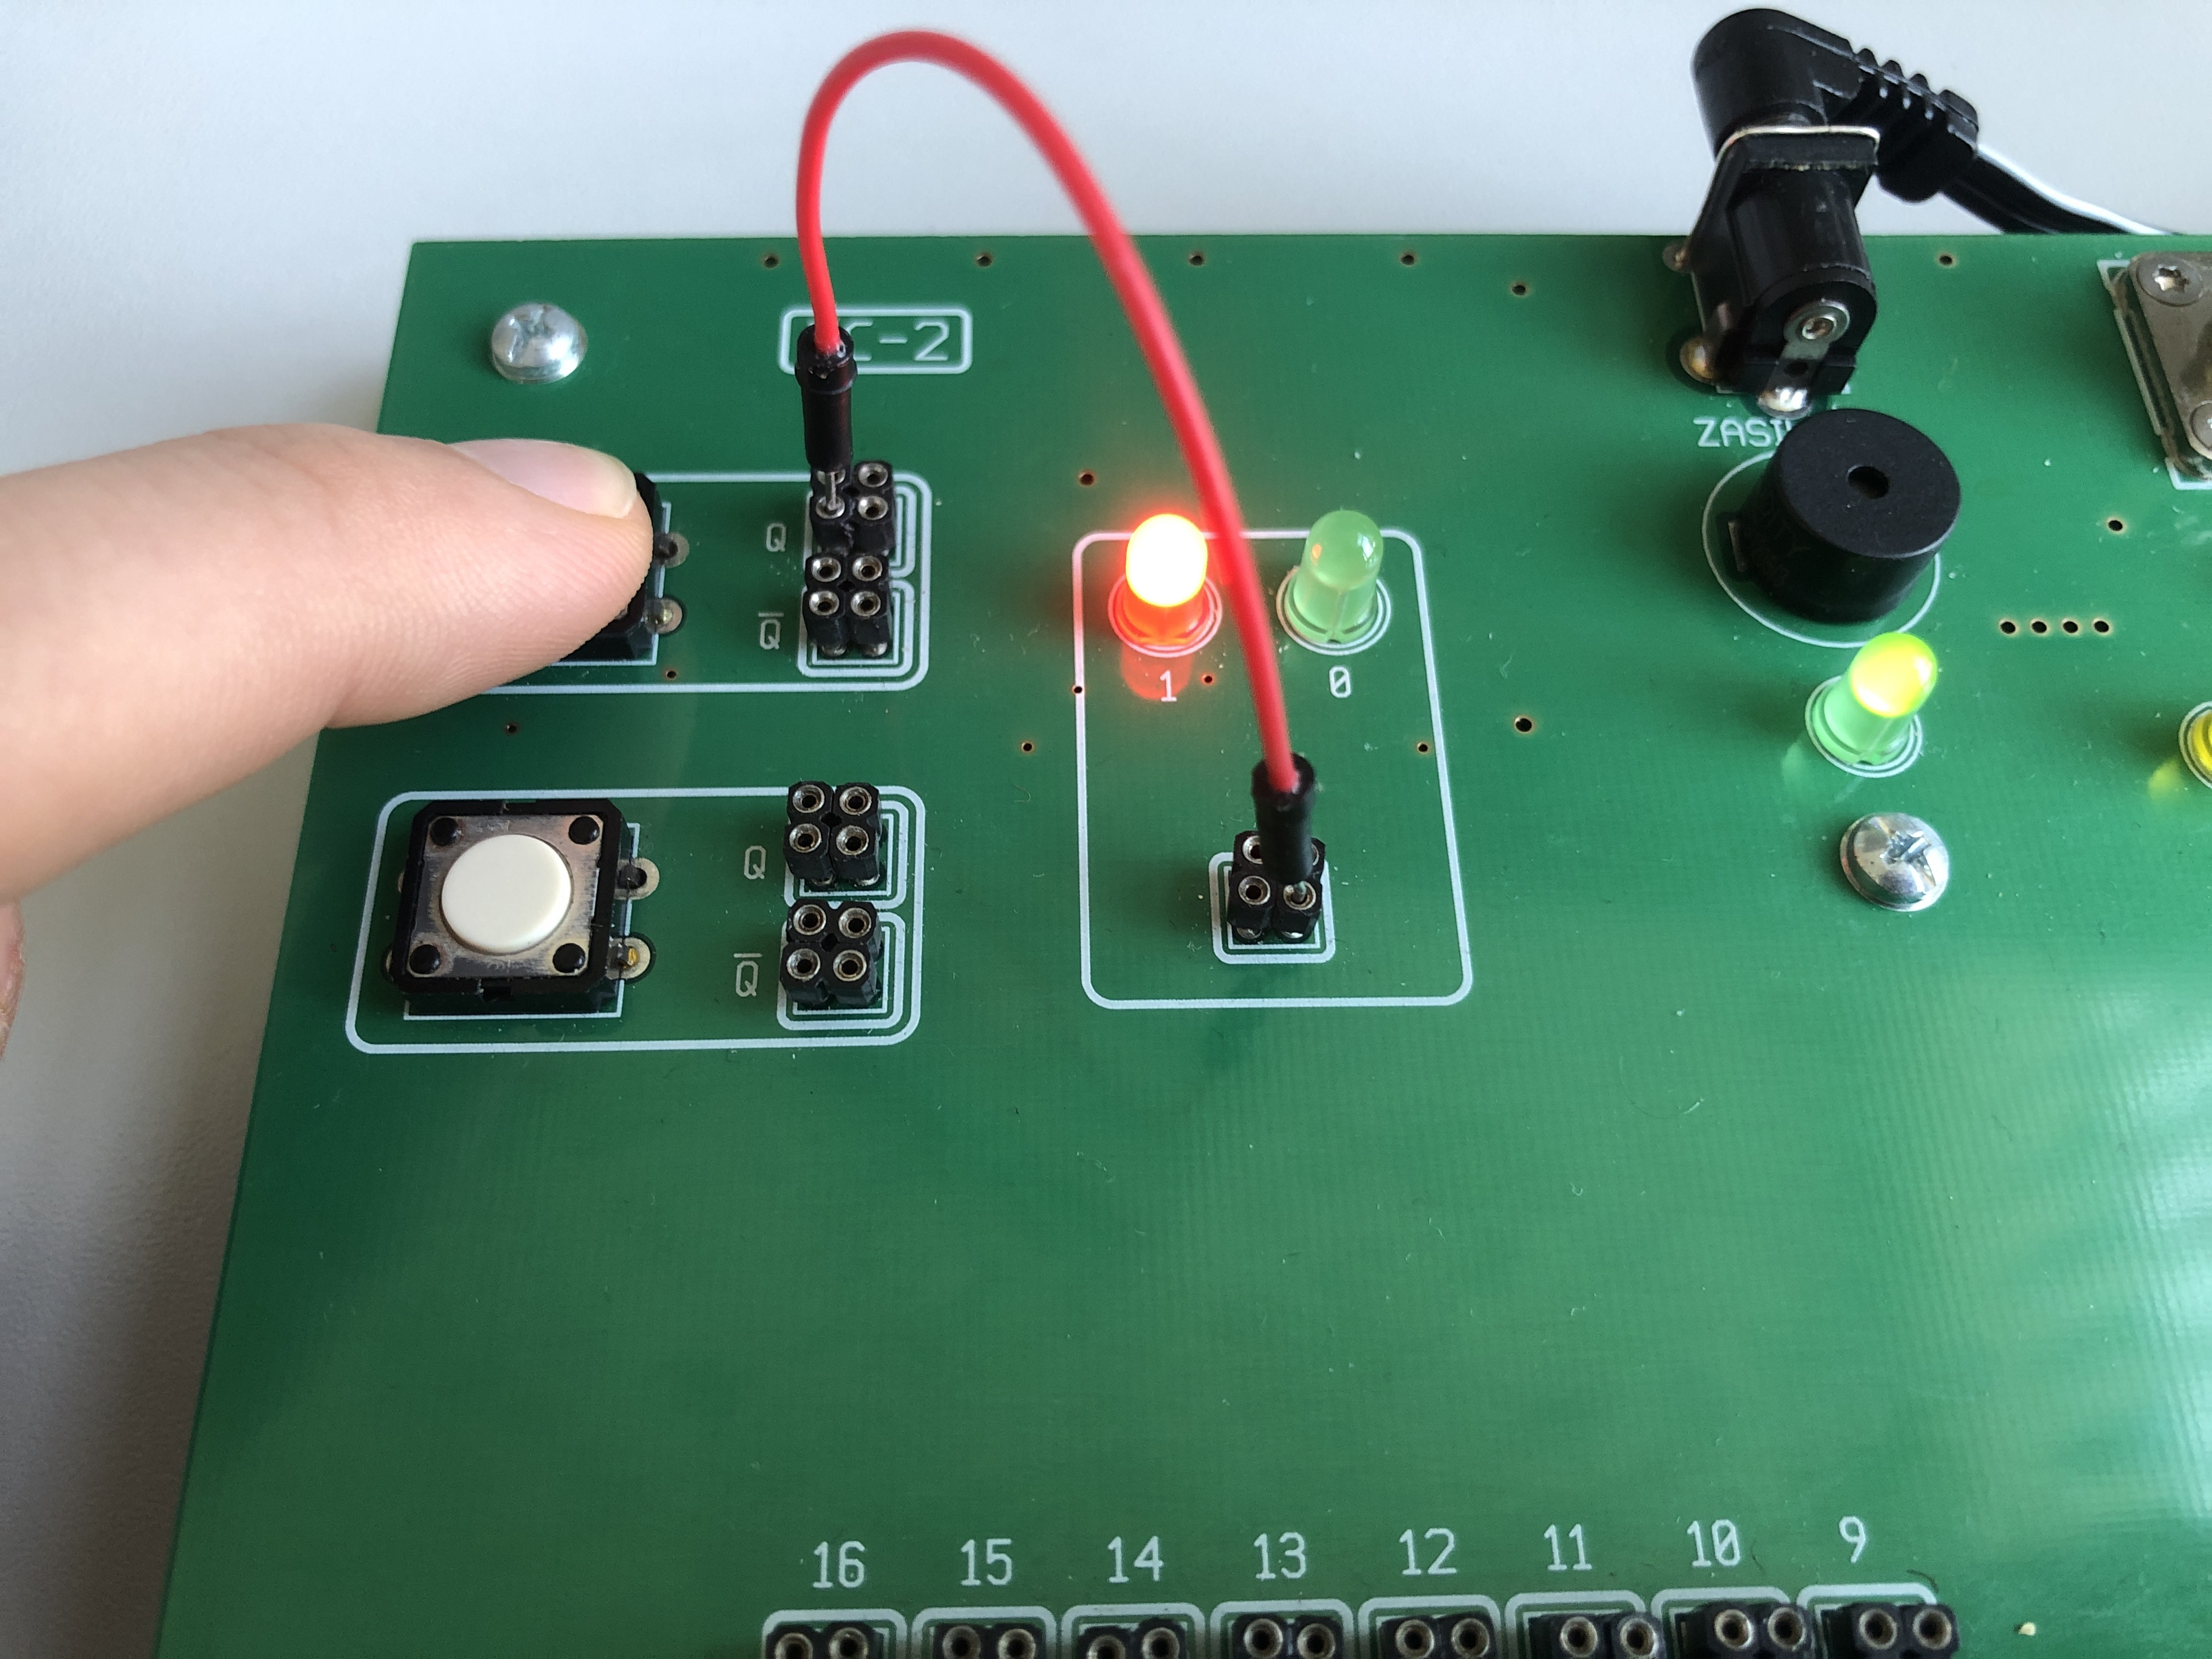
\includegraphics[width=7cm]{C67}}}%
\end{figure}

\newpage
\paragraph{Ćwiczenie 4.2 \\}
Zbadanie tablicy logicznej dla bramek logicznych NAND, NOR i XOR mierząc poziomy napięć na ich wyjściach i sprawdzając je próbnikiem stanów logicznych.


\newpage
\paragraph{Ćwiczenie 4.3 a) \\}
Używając tylko funktorów NAND zbudowanie układu realizującego sumę logiczną (OR), iloczyn logiczny (AND) oraz negację (NOT), sprawdzając ich tablice logiczne używając próbnika stanów logicznych.

\begin{center}
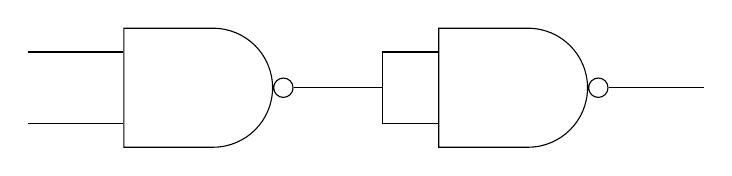
\begin{tikzpicture}[circuit logic US, scale=2]

	\node [nand gate, inputs=nnnn] (gate1) at (0,0) {};
	\node [nand gate, inputs=nnnn] (gate2) at (2,0) {};

	\draw (gate1.output) -- (1.2,0);

	\draw (1.2,0) |- (gate2.input 1);
	\draw (1.2,0) |- (gate2.input 4);

	\draw (gate1.input 1) -- ++(left: 6mm);
	\draw (gate1.input 4) -- ++(left: 6mm);
	\draw (gate2.output) -- ++(right: 6mm);

\end{tikzpicture}
\end{center}

\begin{center}
\begin{tikzpicture}[circuit logic US, scale=2]

	\node [nand gate, inputs=nnnn] (gate3) at (4.4,1) {};
	\draw (gate3.output) -- ++(right: 6mm);

	\node [nand gate, inputs=nnnn] (gate1) at (2,2) {};
	\draw (1.2,2) -- ++(left: 6mm);
	\draw (1.2,2) |- (gate1.input 1);
	\draw (1.2,2) |- (gate1.input 4);
	\draw (gate1.output) -- ++(right: 6mm) |- (gate3.input 1);

	\node [nand gate, inputs=nnnn] (gate2) at (2,0) {};
	\draw (1.2,0) -- ++(left: 6mm);
	\draw (1.2,0) |- (gate2.input 1);
	\draw (1.2,0) |- (gate2.input 4);
	\draw (gate2.output) -- ++(right: 6mm) |- (gate3.input 4);
	
\end{tikzpicture}
\end{center}

\begin{center}
\begin{tikzpicture}[circuit logic US, scale=2]

	\node [nand gate, inputs=nnnn] (gate2) at (2,0) {};

	\draw (1.2,0) -- ++(left: 6mm);

	\draw (1.2,0) |- (gate2.input 1);
	\draw (1.2,0) |- (gate2.input 4);

	\draw (gate2.output) -- ++(right: 6mm);

\end{tikzpicture}
\end{center}

\newpage
\paragraph{Ćwiczenie 4.3 b) \\}
Używając tylko funktorów NOR zbudowanie układu realizującego sumę logiczną (OR), iloczyn logiczny (AND) oraz negację (NOT), sprawdzając ich tablice logiczne używając próbnika stanów logicznych.


\begin{center}
\begin{tikzpicture}[circuit logic US, scale=2]

	\node [nor gate, inputs=nnnn] (gate3) at (4.4,1) {};
	\draw (gate3.output) -- ++(right: 6mm);

	\node [nor gate, inputs=nnnn] (gate1) at (2,2) {};
	\draw (1.2,2) -- ++(left: 6mm);
	\draw (1.2,2) |- (gate1.input 1);
	\draw (1.2,2) |- (gate1.input 4);
	\draw (gate1.output) -- ++(right: 6mm) |- (gate3.input 1);

	\node [nor gate, inputs=nnnn] (gate2) at (2,0) {};
	\draw (1.2,0) -- ++(left: 6mm);
	\draw (1.2,0) |- (gate2.input 1);
	\draw (1.2,0) |- (gate2.input 4);
	\draw (gate2.output) -- ++(right: 6mm) |- (gate3.input 4);
	
\end{tikzpicture}
\end{center}

\begin{center}
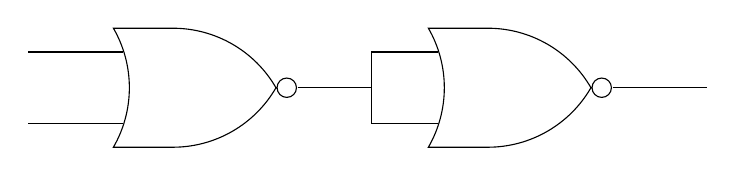
\begin{tikzpicture}[circuit logic US, scale=2]

	\node [nor gate, inputs=nnnn] (gate1) at (0,0) {};
	\node [nor gate, inputs=nnnn] (gate2) at (2,0) {};

	\draw (gate1.output) -- (1.2,0);

	\draw (1.2,0) |- (gate2.input 1);
	\draw (1.2,0) |- (gate2.input 4);

	\draw (gate1.input 1) -- ++(left: 6mm);
	\draw (gate1.input 4) -- ++(left: 6mm);
	\draw (gate2.output) -- ++(right: 6mm);

\end{tikzpicture}
\end{center}

\begin{center}
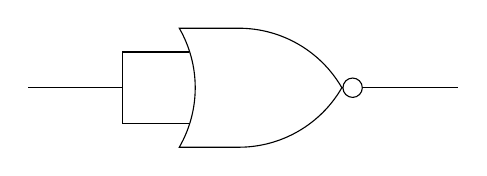
\begin{tikzpicture}[circuit logic US, scale=2]

	\node [nor gate, inputs=nnnn] (gate2) at (2,0) {};

	\draw (1.2,0) -- ++(left: 6mm);

	\draw (1.2,0) |- (gate2.input 1);
	\draw (1.2,0) |- (gate2.input 4);

	\draw (gate2.output) -- ++(right: 6mm);

\end{tikzpicture}
\end{center}


\newpage
\paragraph{Ćwiczenie 4.4 \\}
Zmontowanie generatora zbudowanego z trzech bramek NAND. Zmie- rzenie średniego czasu propagacji impulsu przez bramkę mierząc okres drgań generatora. Porównać czasy propagacji bramek NAND na układach scalonych serii podstawowej 7400 i bramek z serii szybkiej 74S00.

\begin{center}
\begin{tikzpicture}[circuit logic US, scale=2]

	\node [nand gate, inputs=nnnn] (nand1) at (0,0) {};
	\node [nand gate, inputs=nnnn] (nand2) at (2,0) {};
	\node [nand gate, inputs=nnnn] (nand3) at (4,0) {};

	\draw (nand1.output) -- (1.2,0);
	\draw (nand2.output) -- (3.2,0);
	\draw (nand3.output) -- (5.2,0);

	\draw (-1.4,0) -- (-0.8,0) |- (nand1.input 1);
	\draw (-0.8,0) |- (nand1.input 4);

	\draw (1.2,0) |- (nand2.input 1);
	\draw (1.2,0) |- (nand2.input 4);

	\draw (3.2,0) |- (nand3.input 1);
	\draw (3.2,0) |- (nand3.input 4);

	\draw (5.2,0) -- (5.2,1) -- (-1.4,1) -- (-1.4,0);
	\draw (5.2,0) -- node[at end, right]{WY} (5.8,0);
	
\end{tikzpicture}
\end{center}


\newpage
\paragraph{Ćwiczenie 4.5 \\}
Zbudowanie układu realizującego funkcję logiczną dla jednego segmentu wyświetlacza 7-segmentowego, którego zadaniem będzie wyświetlanie liczb w systemie ósemkowym.

\begin{center}
\begin{tikzpicture}[circuit logic US, scale=2]

	\node [nand gate, inputs=nnnn] (nand1) at (4,0) {};
	\node [nor gate, inputs=nnnn] (nor1) at (0,1) {};

	\draw (nand1.output) -- ++(right: 8mm);
	\draw (nor1.output) -- ++(right: 12mm) |- (nand1.input 1);
	\draw (nand1.input 4) -- node[at end, left]{B} ++(left: 54.5mm);
	\draw (nor1.input 1) -- node[at end, left]{D} ++(left: 15mm);
	\draw (nor1.input 4) -- node[at end, left]{C} ++(left: 15mm);

\end{tikzpicture}
\end{center}


\newpage
\paragraph{Ćwiczenie 4.6 \\}
Zaprojektowanie i zmontowanie przerzutnika asynchronicznego R-S z funktorów NAND i sprawdzenie tablicy przejść.

\begin{center}
\begin{tikzpicture}[circuit logic US, scale=2]

	\node [nand gate, inputs=nnnn] (nand1) at (0, 0) {};
	\node [nand gate, inputs=nnnn] (nand2) at (0, -2) {};

	\draw (nand1.input 1) -- node[at end, left]{S} ++(left: 1cm);
	\draw (nand1.input 4) -- ++(left: 5mm) -- ++(down: 5mm) -- (2,-1.7) -- (2,-2);
	\draw (nand1.output) -- ++(right: 4mm) -- (2,0) -- node[at end, right]{$Q$} ++(right: 1cm);

	\draw (nand2.input 4) -- node[at end, left]{R} ++(left: 1cm);
	\draw (nand2.input 1) -- ++(left: 5mm) -- ++(up: 5mm) -- (2,-0.3) -- (2,0);
	\draw (nand2.output) -- ++(right: 4mm) -- (2,-2) -- node[at end, right]{$\overline{Q}$} ++(right: 1cm);

\end{tikzpicture}
\end{center}




\newpage
\paragraph{Notatki z zeszytu labolatoryjnego \\}
Poniżej załączone są notatki z zeszytu labolatoryjnego, które prowadziłem podczas zajęć wykonując pomiary.

\begin{figure}[H]
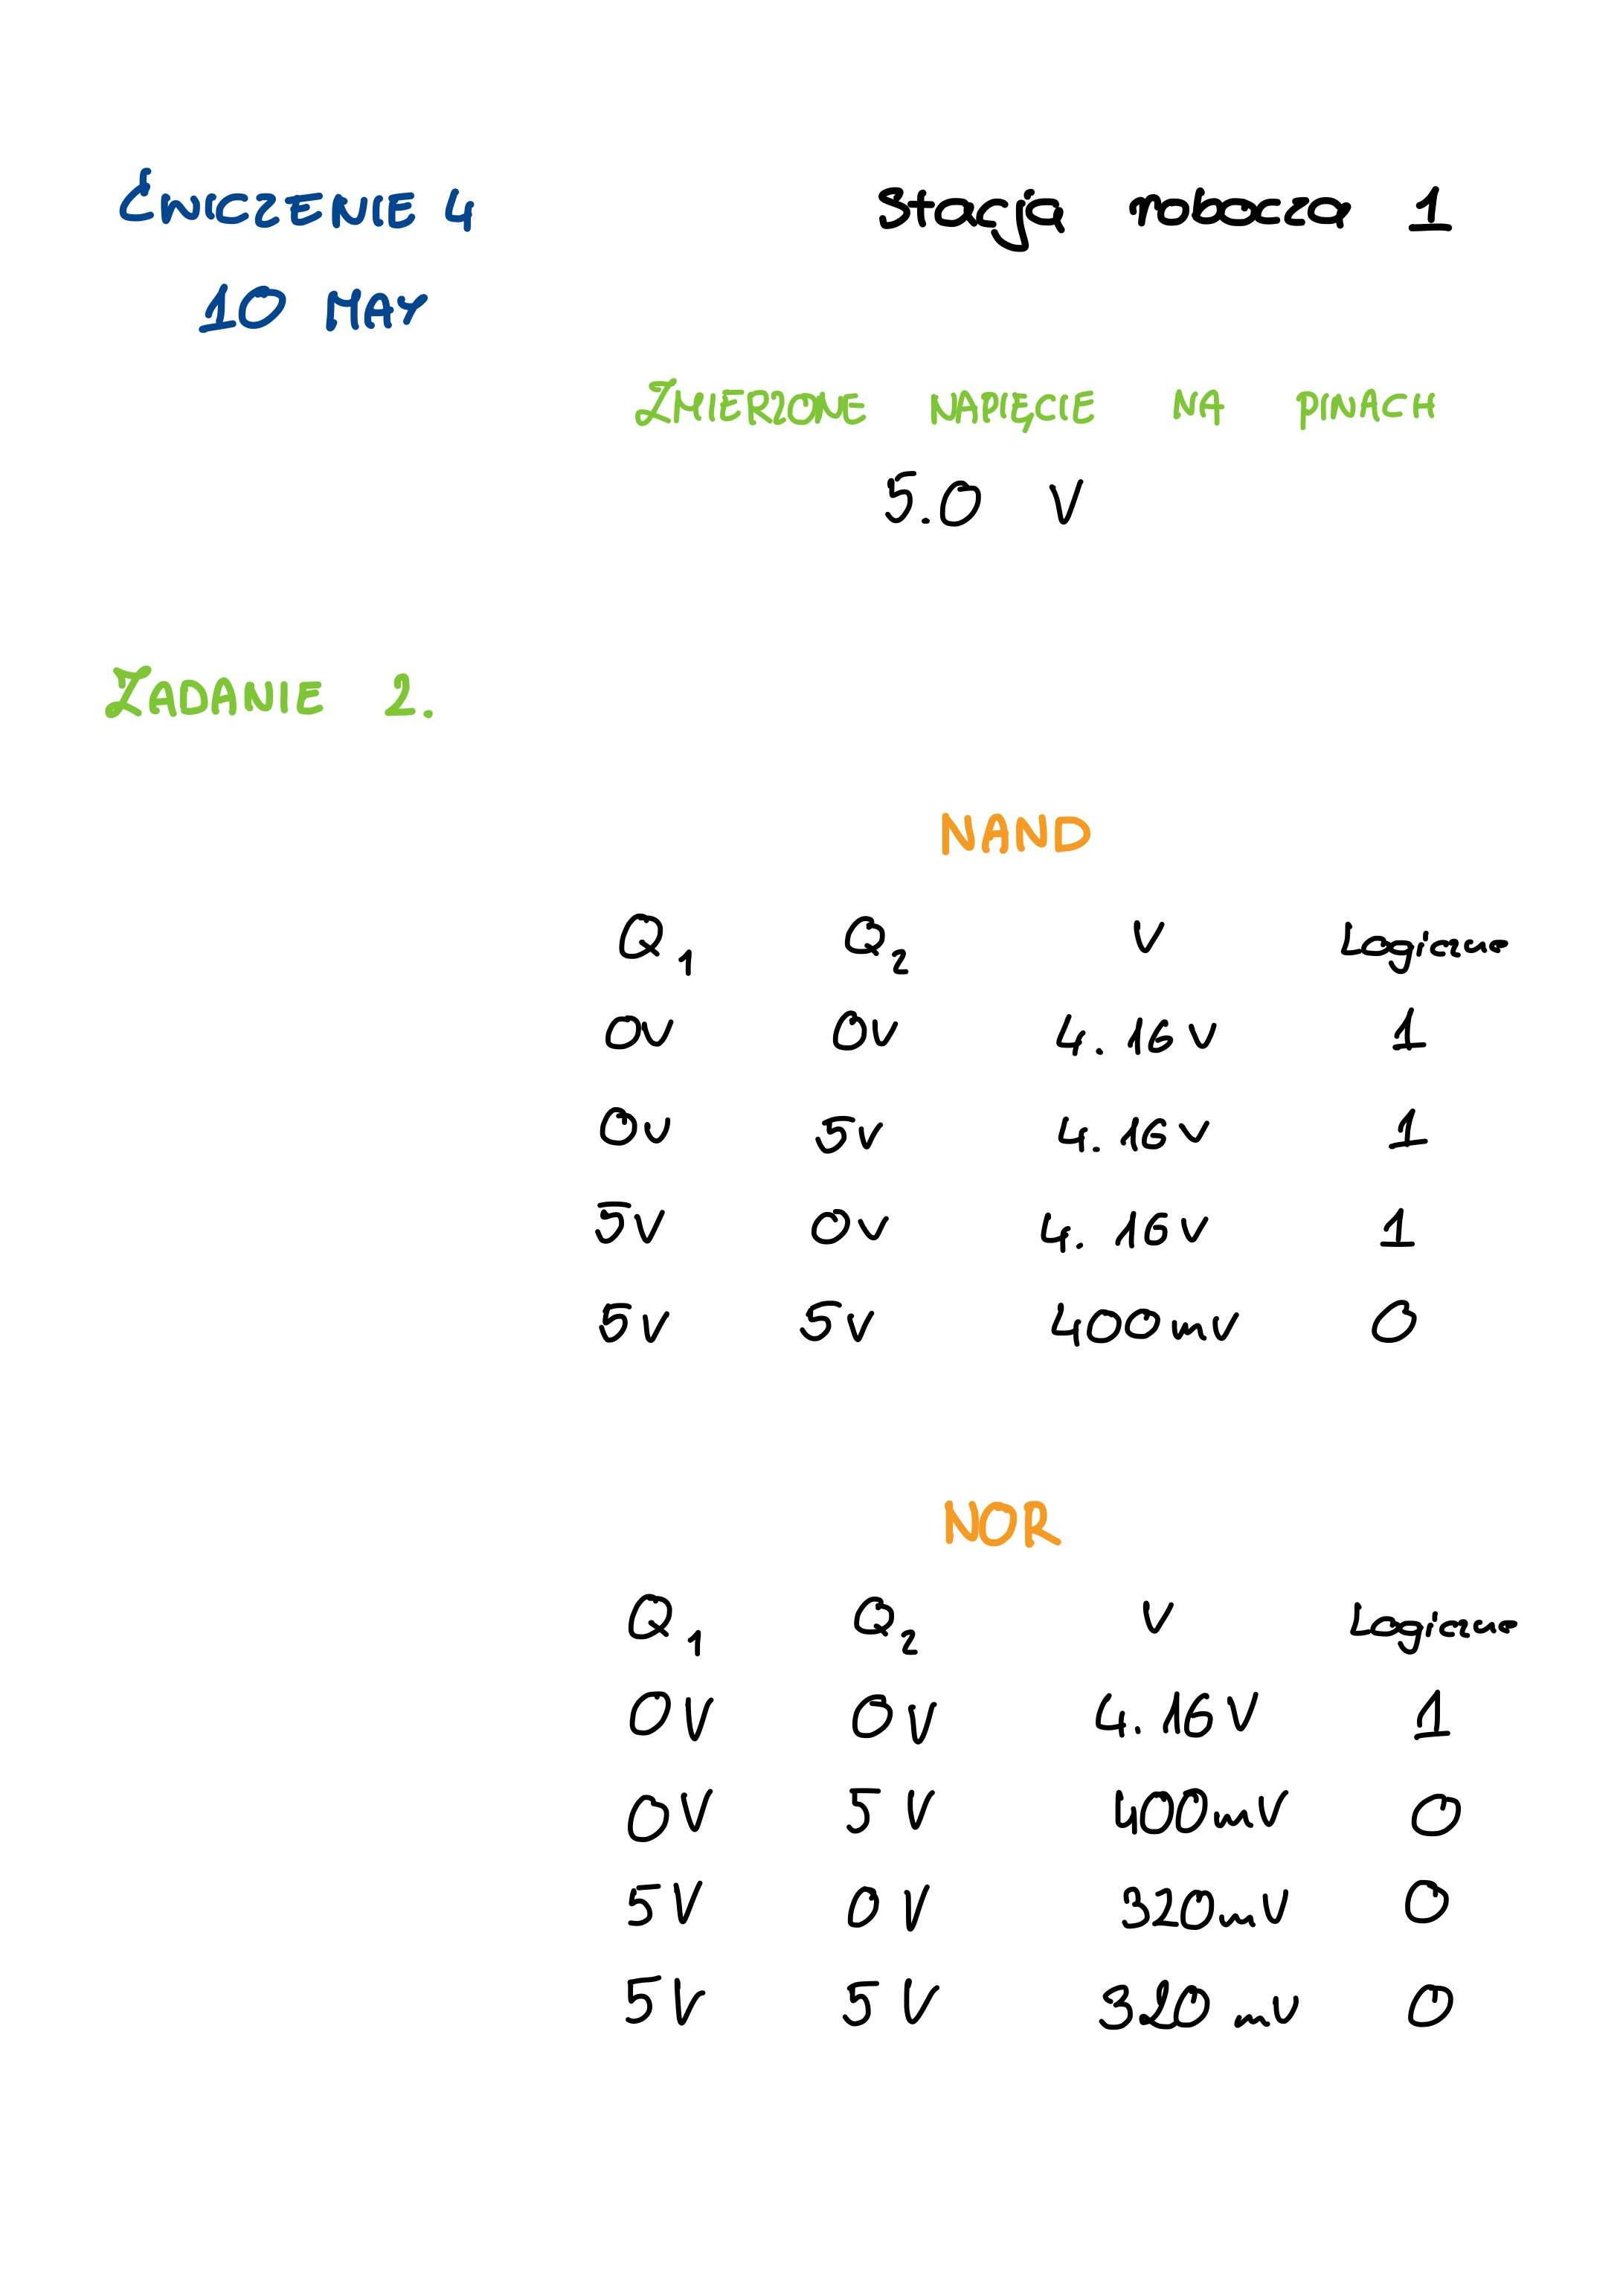
\includegraphics[scale=0.2]{B0}
\centering
\captionsetup{labelformat=empty}
\caption{}
\end{figure}

\begin{figure}[H]
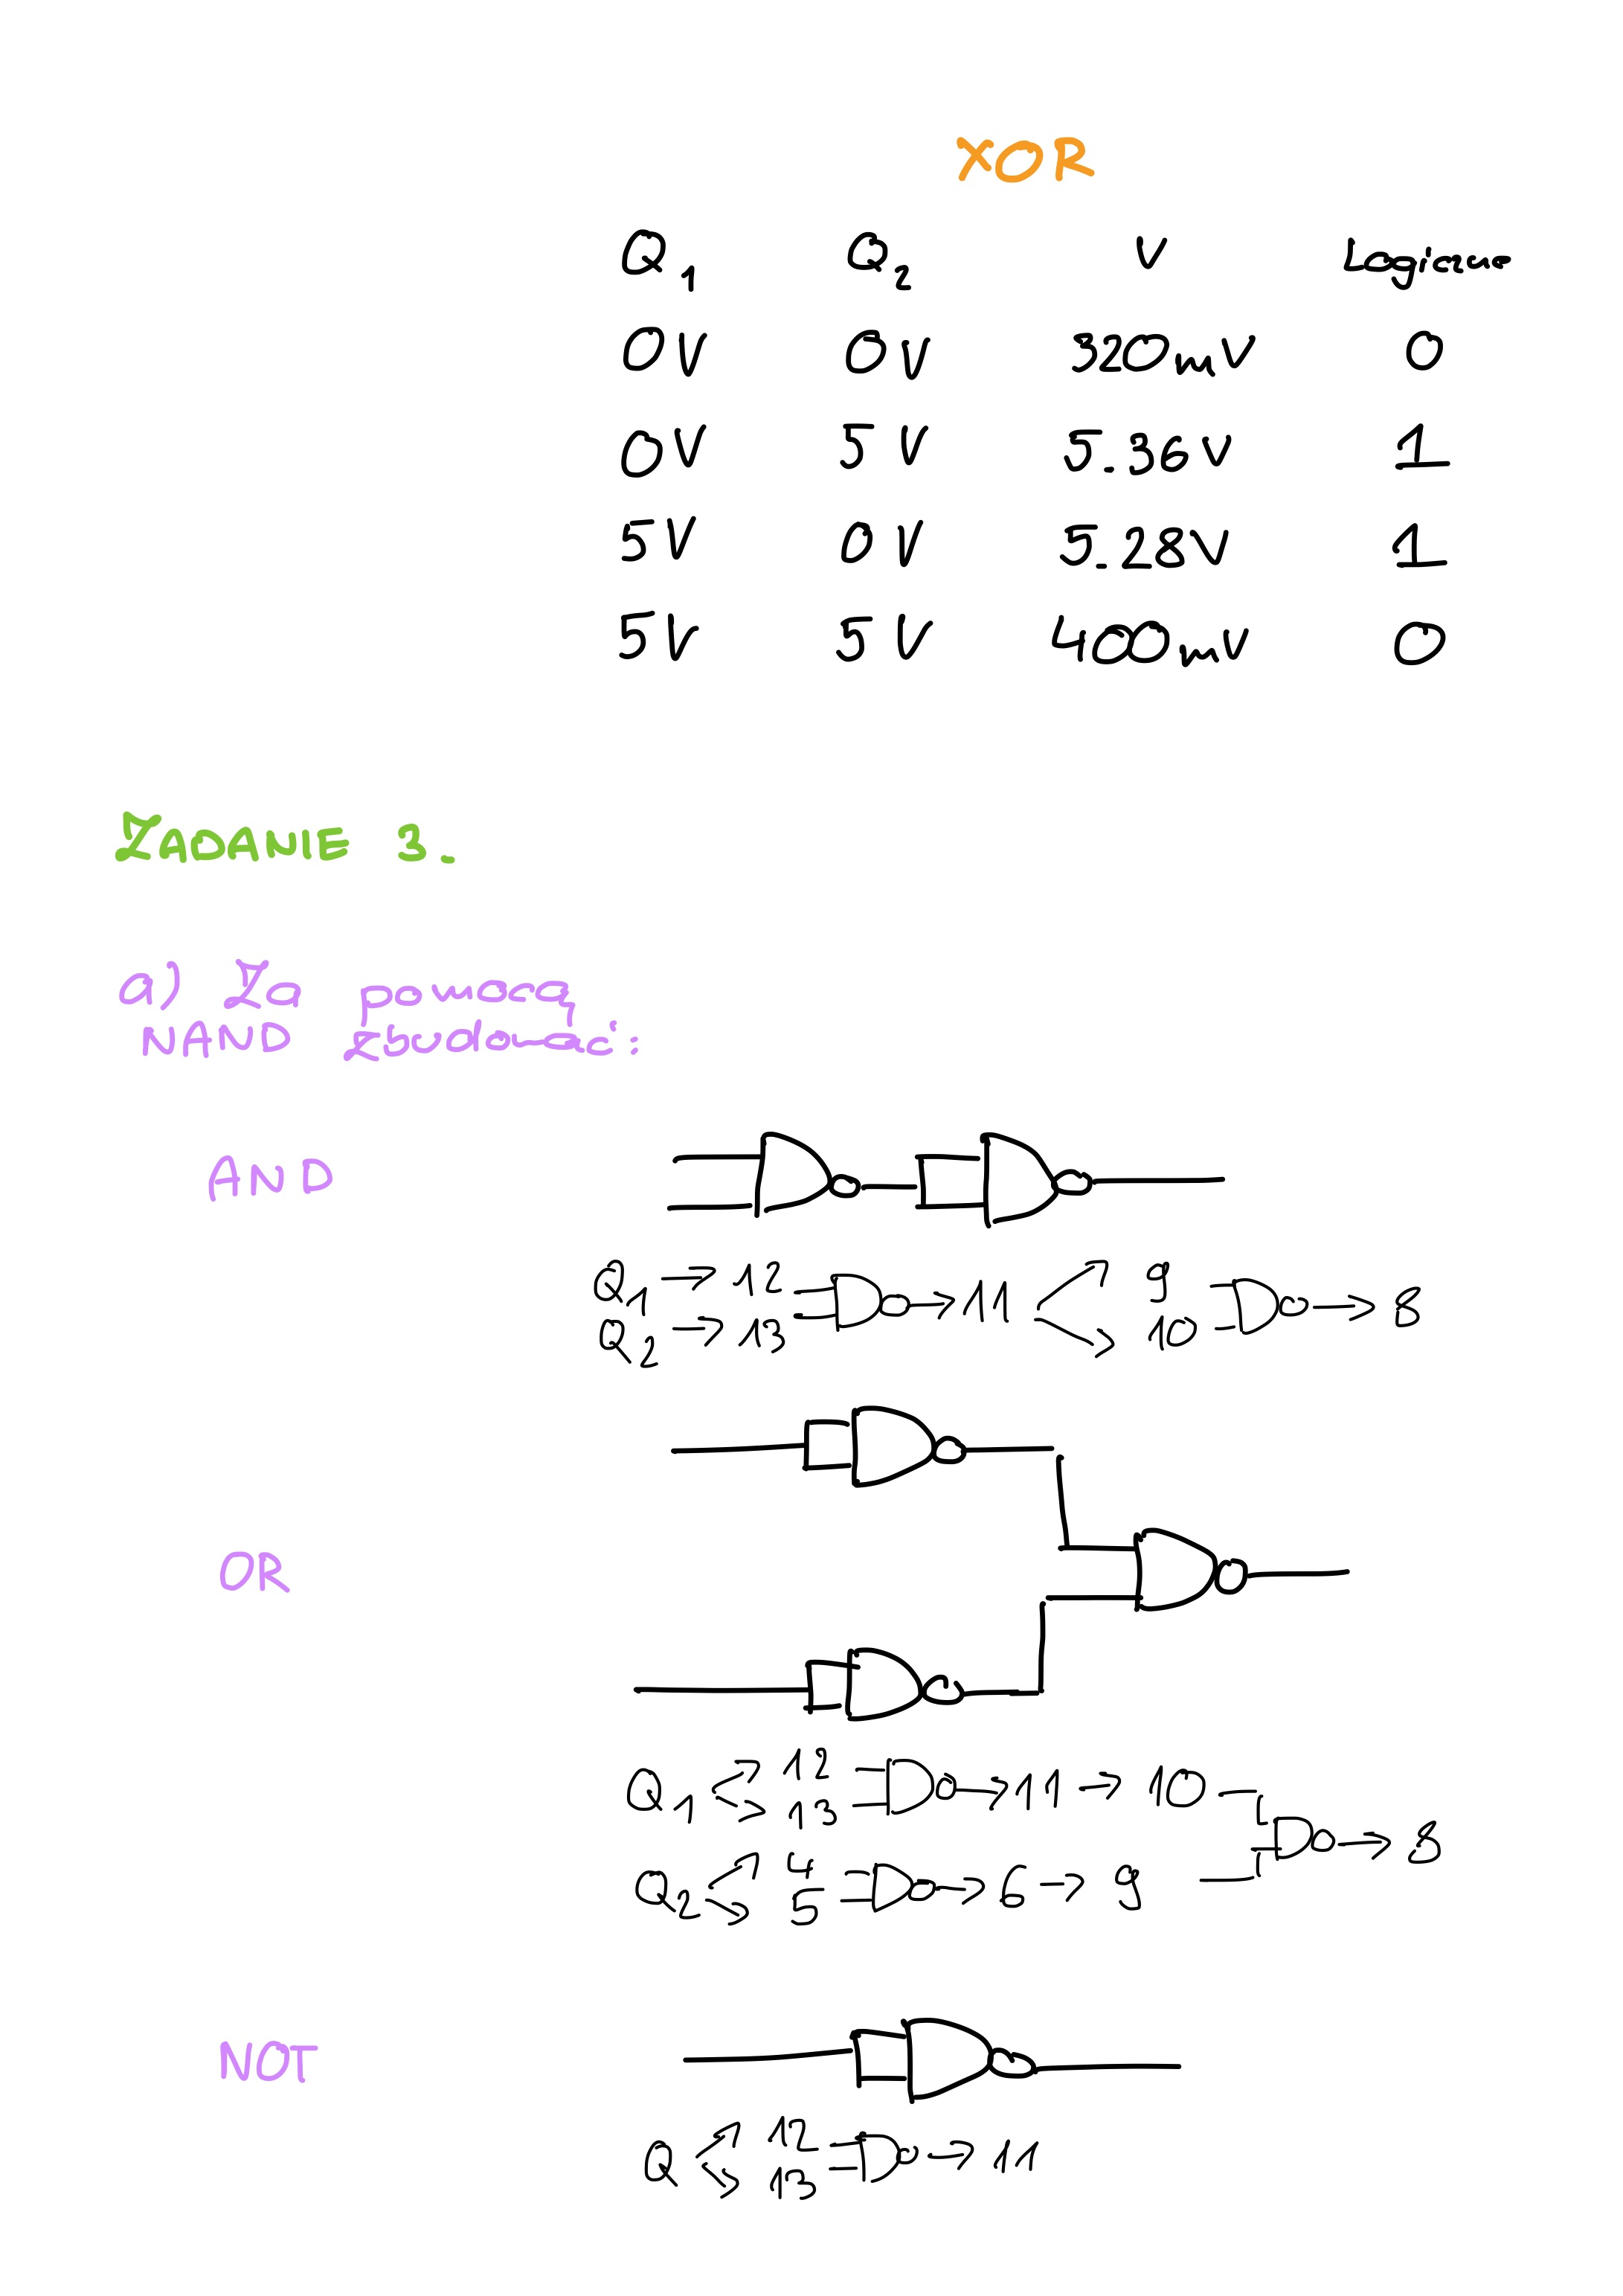
\includegraphics[scale=0.2]{B1}
\centering
\captionsetup{labelformat=empty}
\caption{}
\end{figure}

\begin{figure}[H]
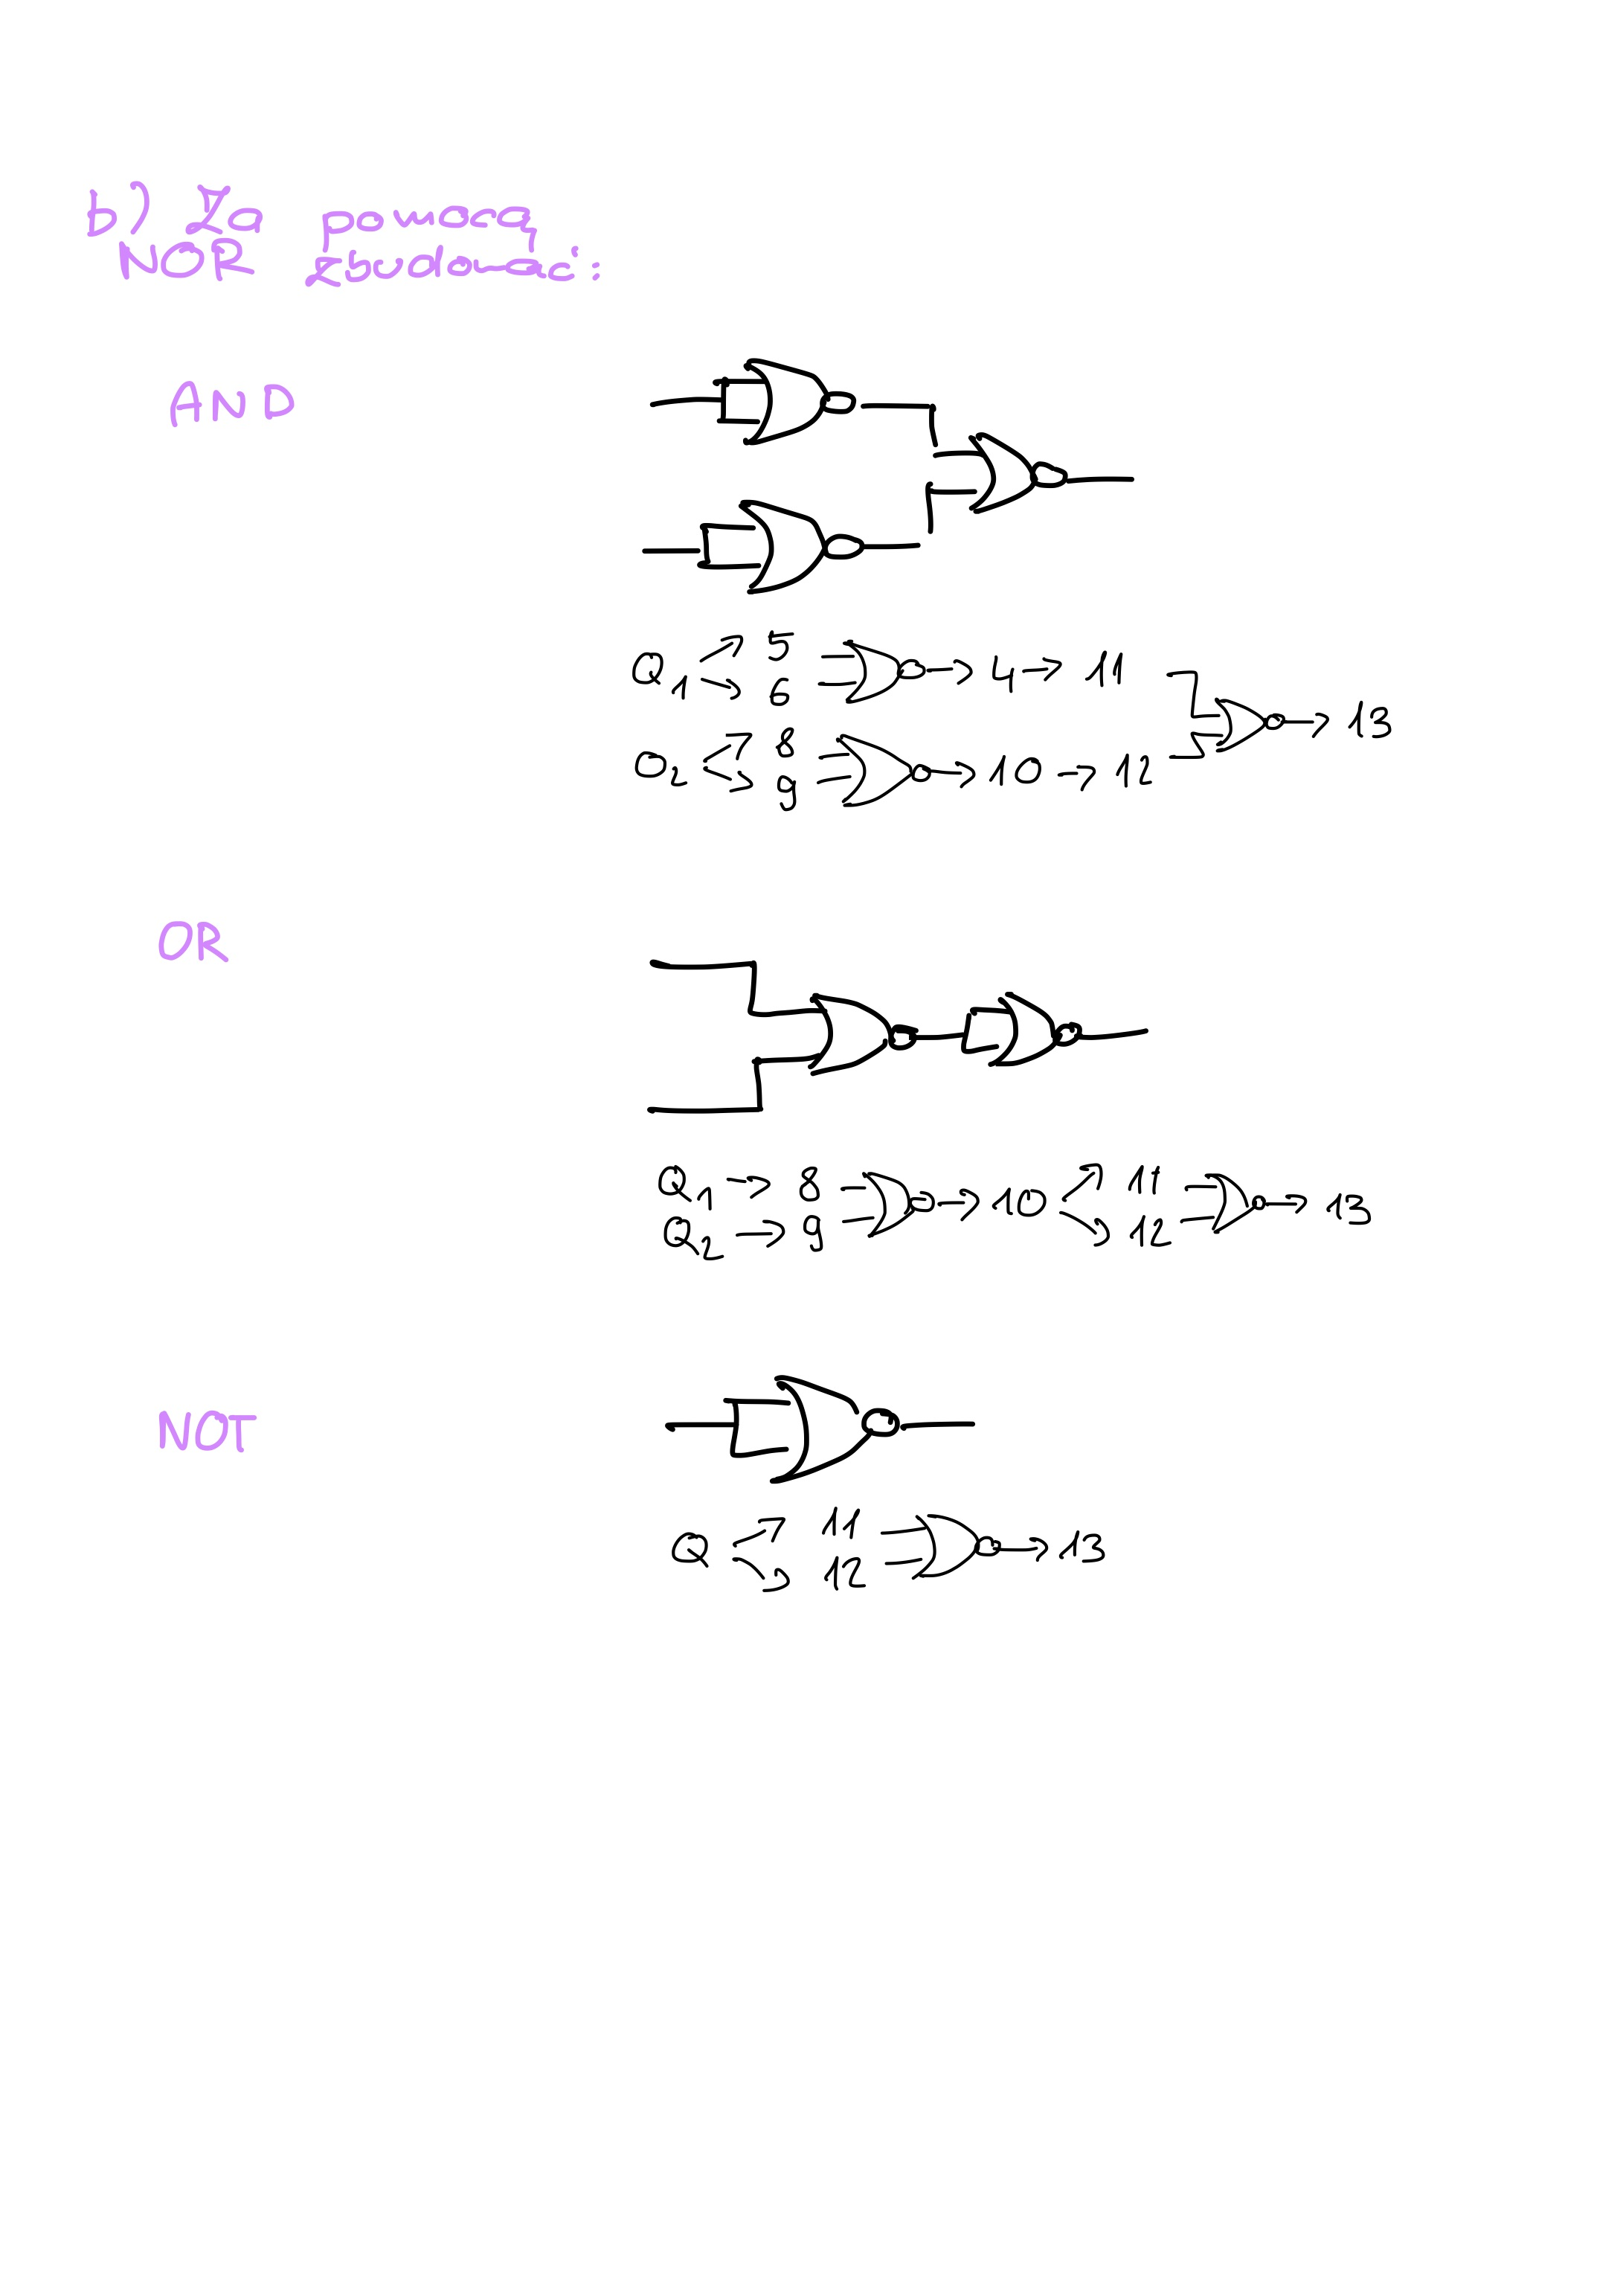
\includegraphics[scale=0.2]{B2}
\centering
\captionsetup{labelformat=empty}
\caption{}
\end{figure}

\begin{figure}[H]
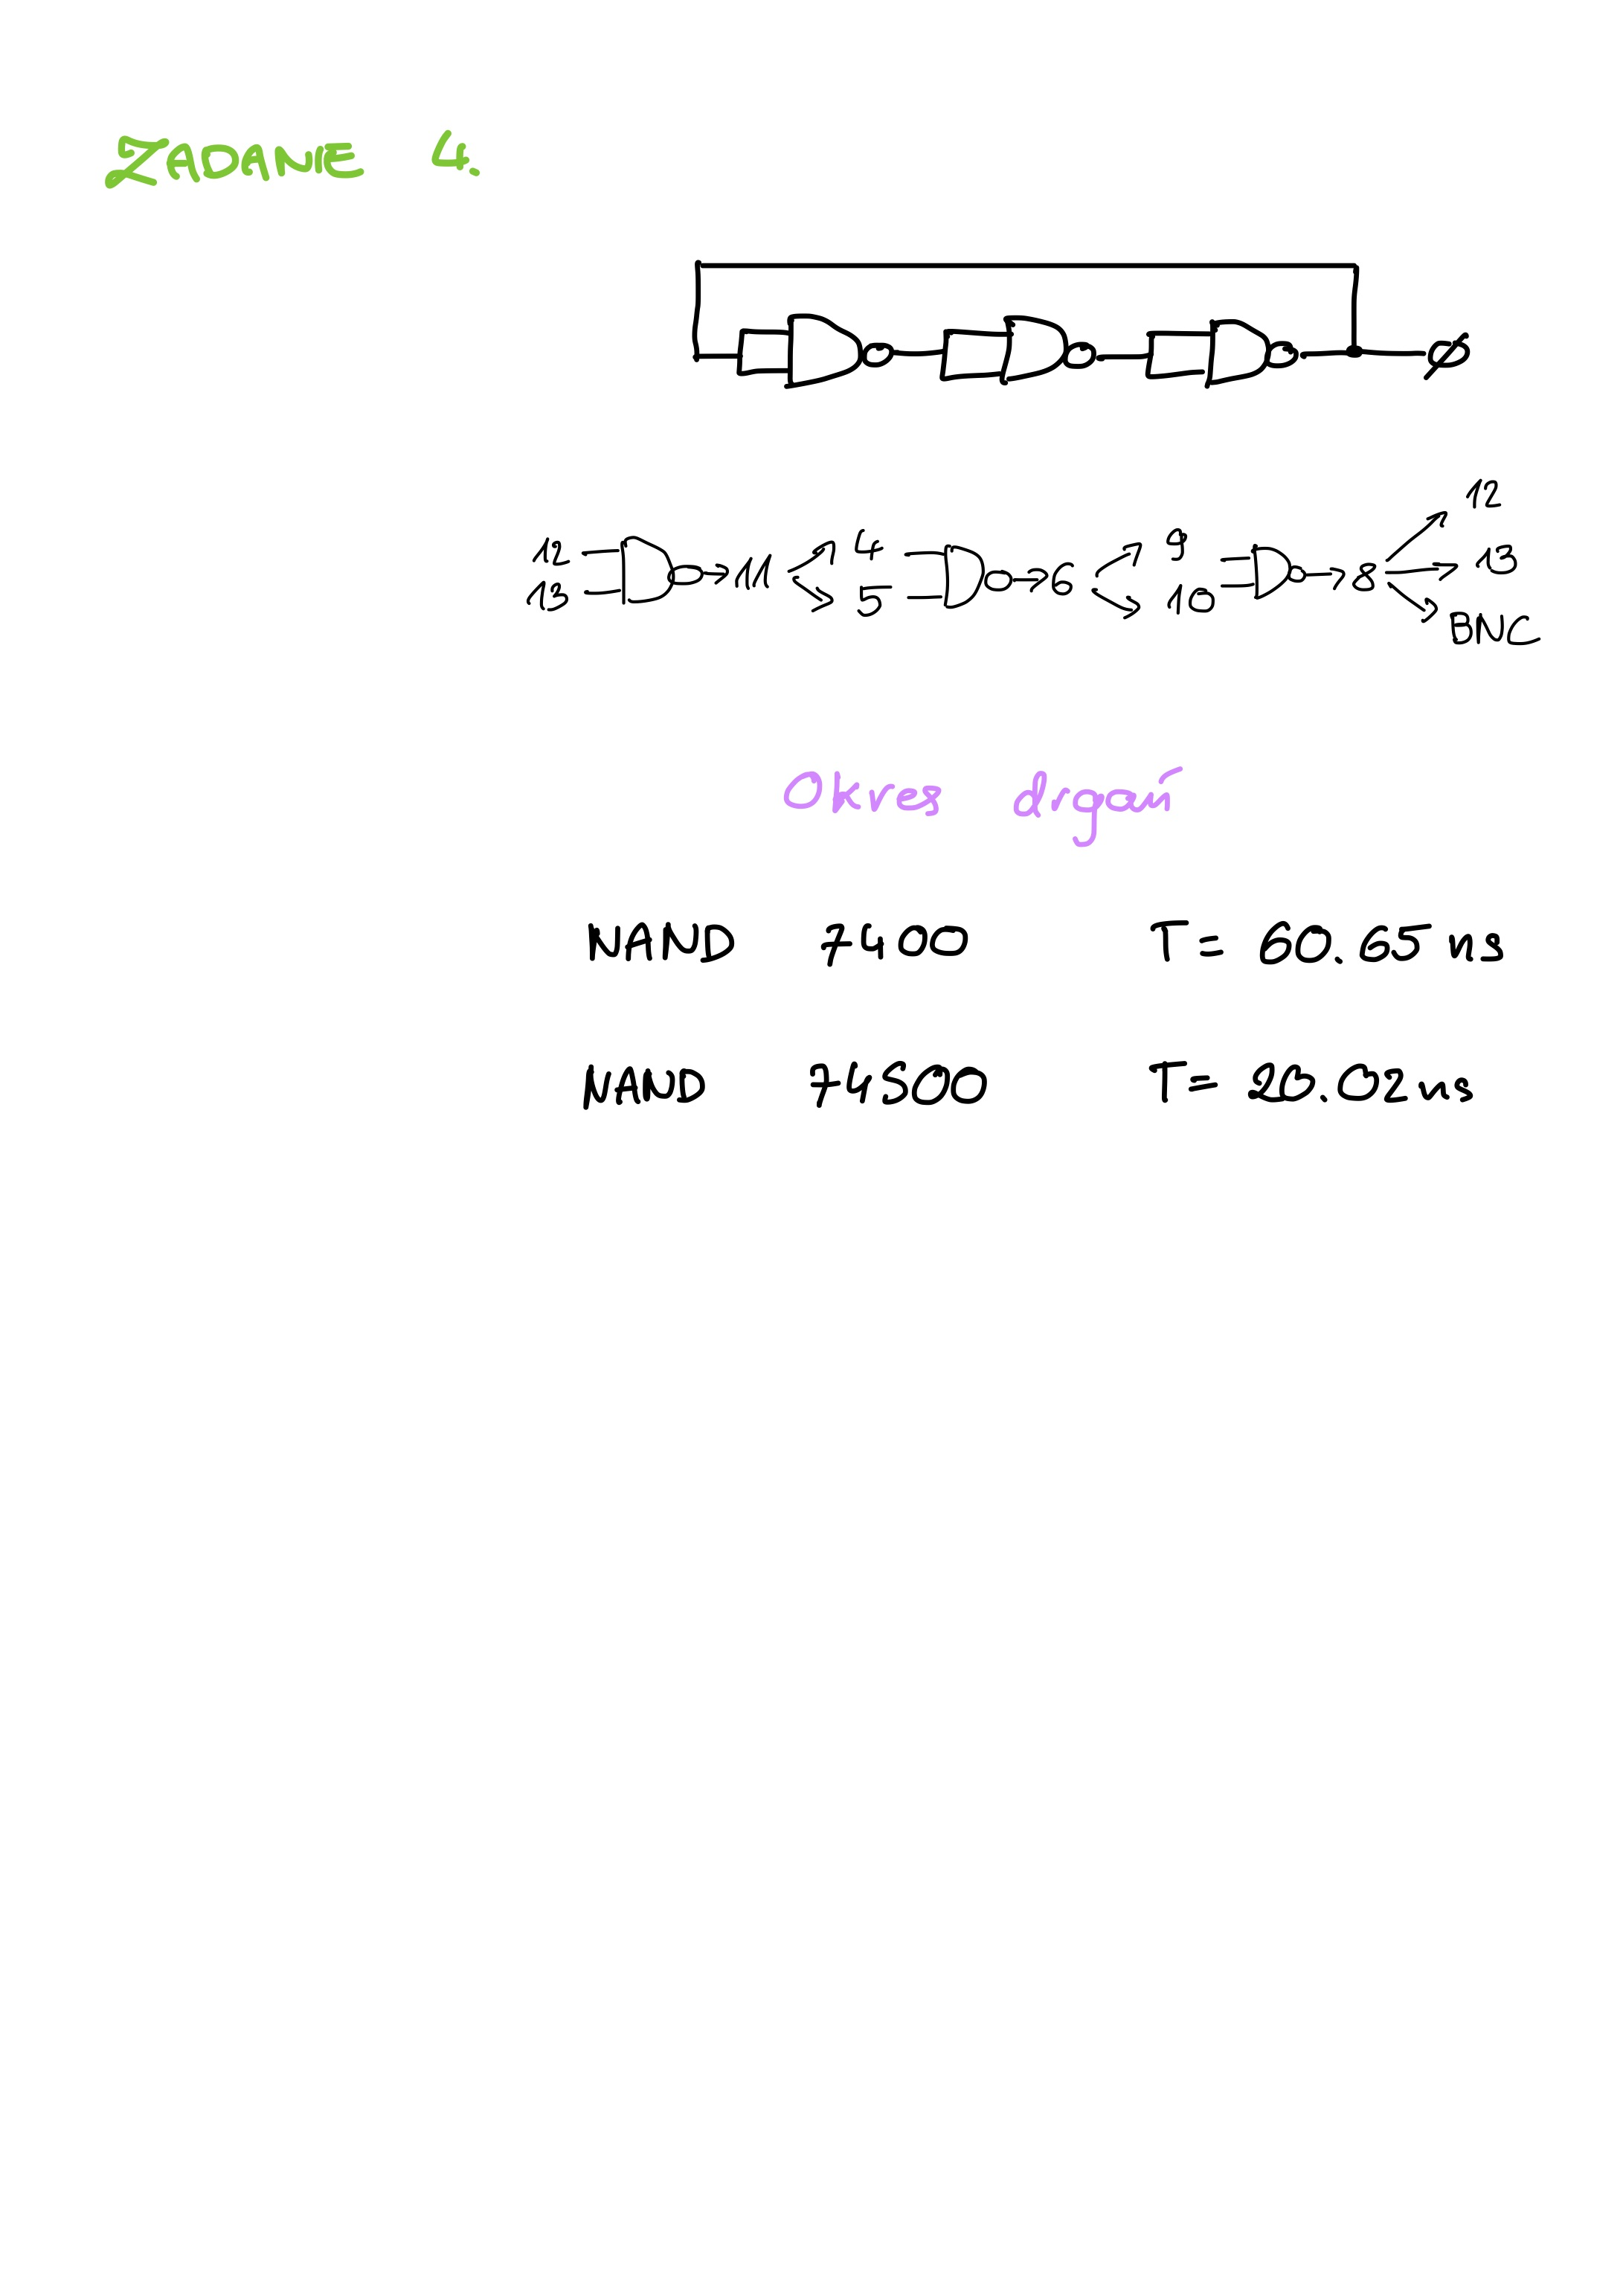
\includegraphics[scale=0.2]{B3}
\centering
\captionsetup{labelformat=empty}
\caption{}
\end{figure}

\begin{figure}[H]
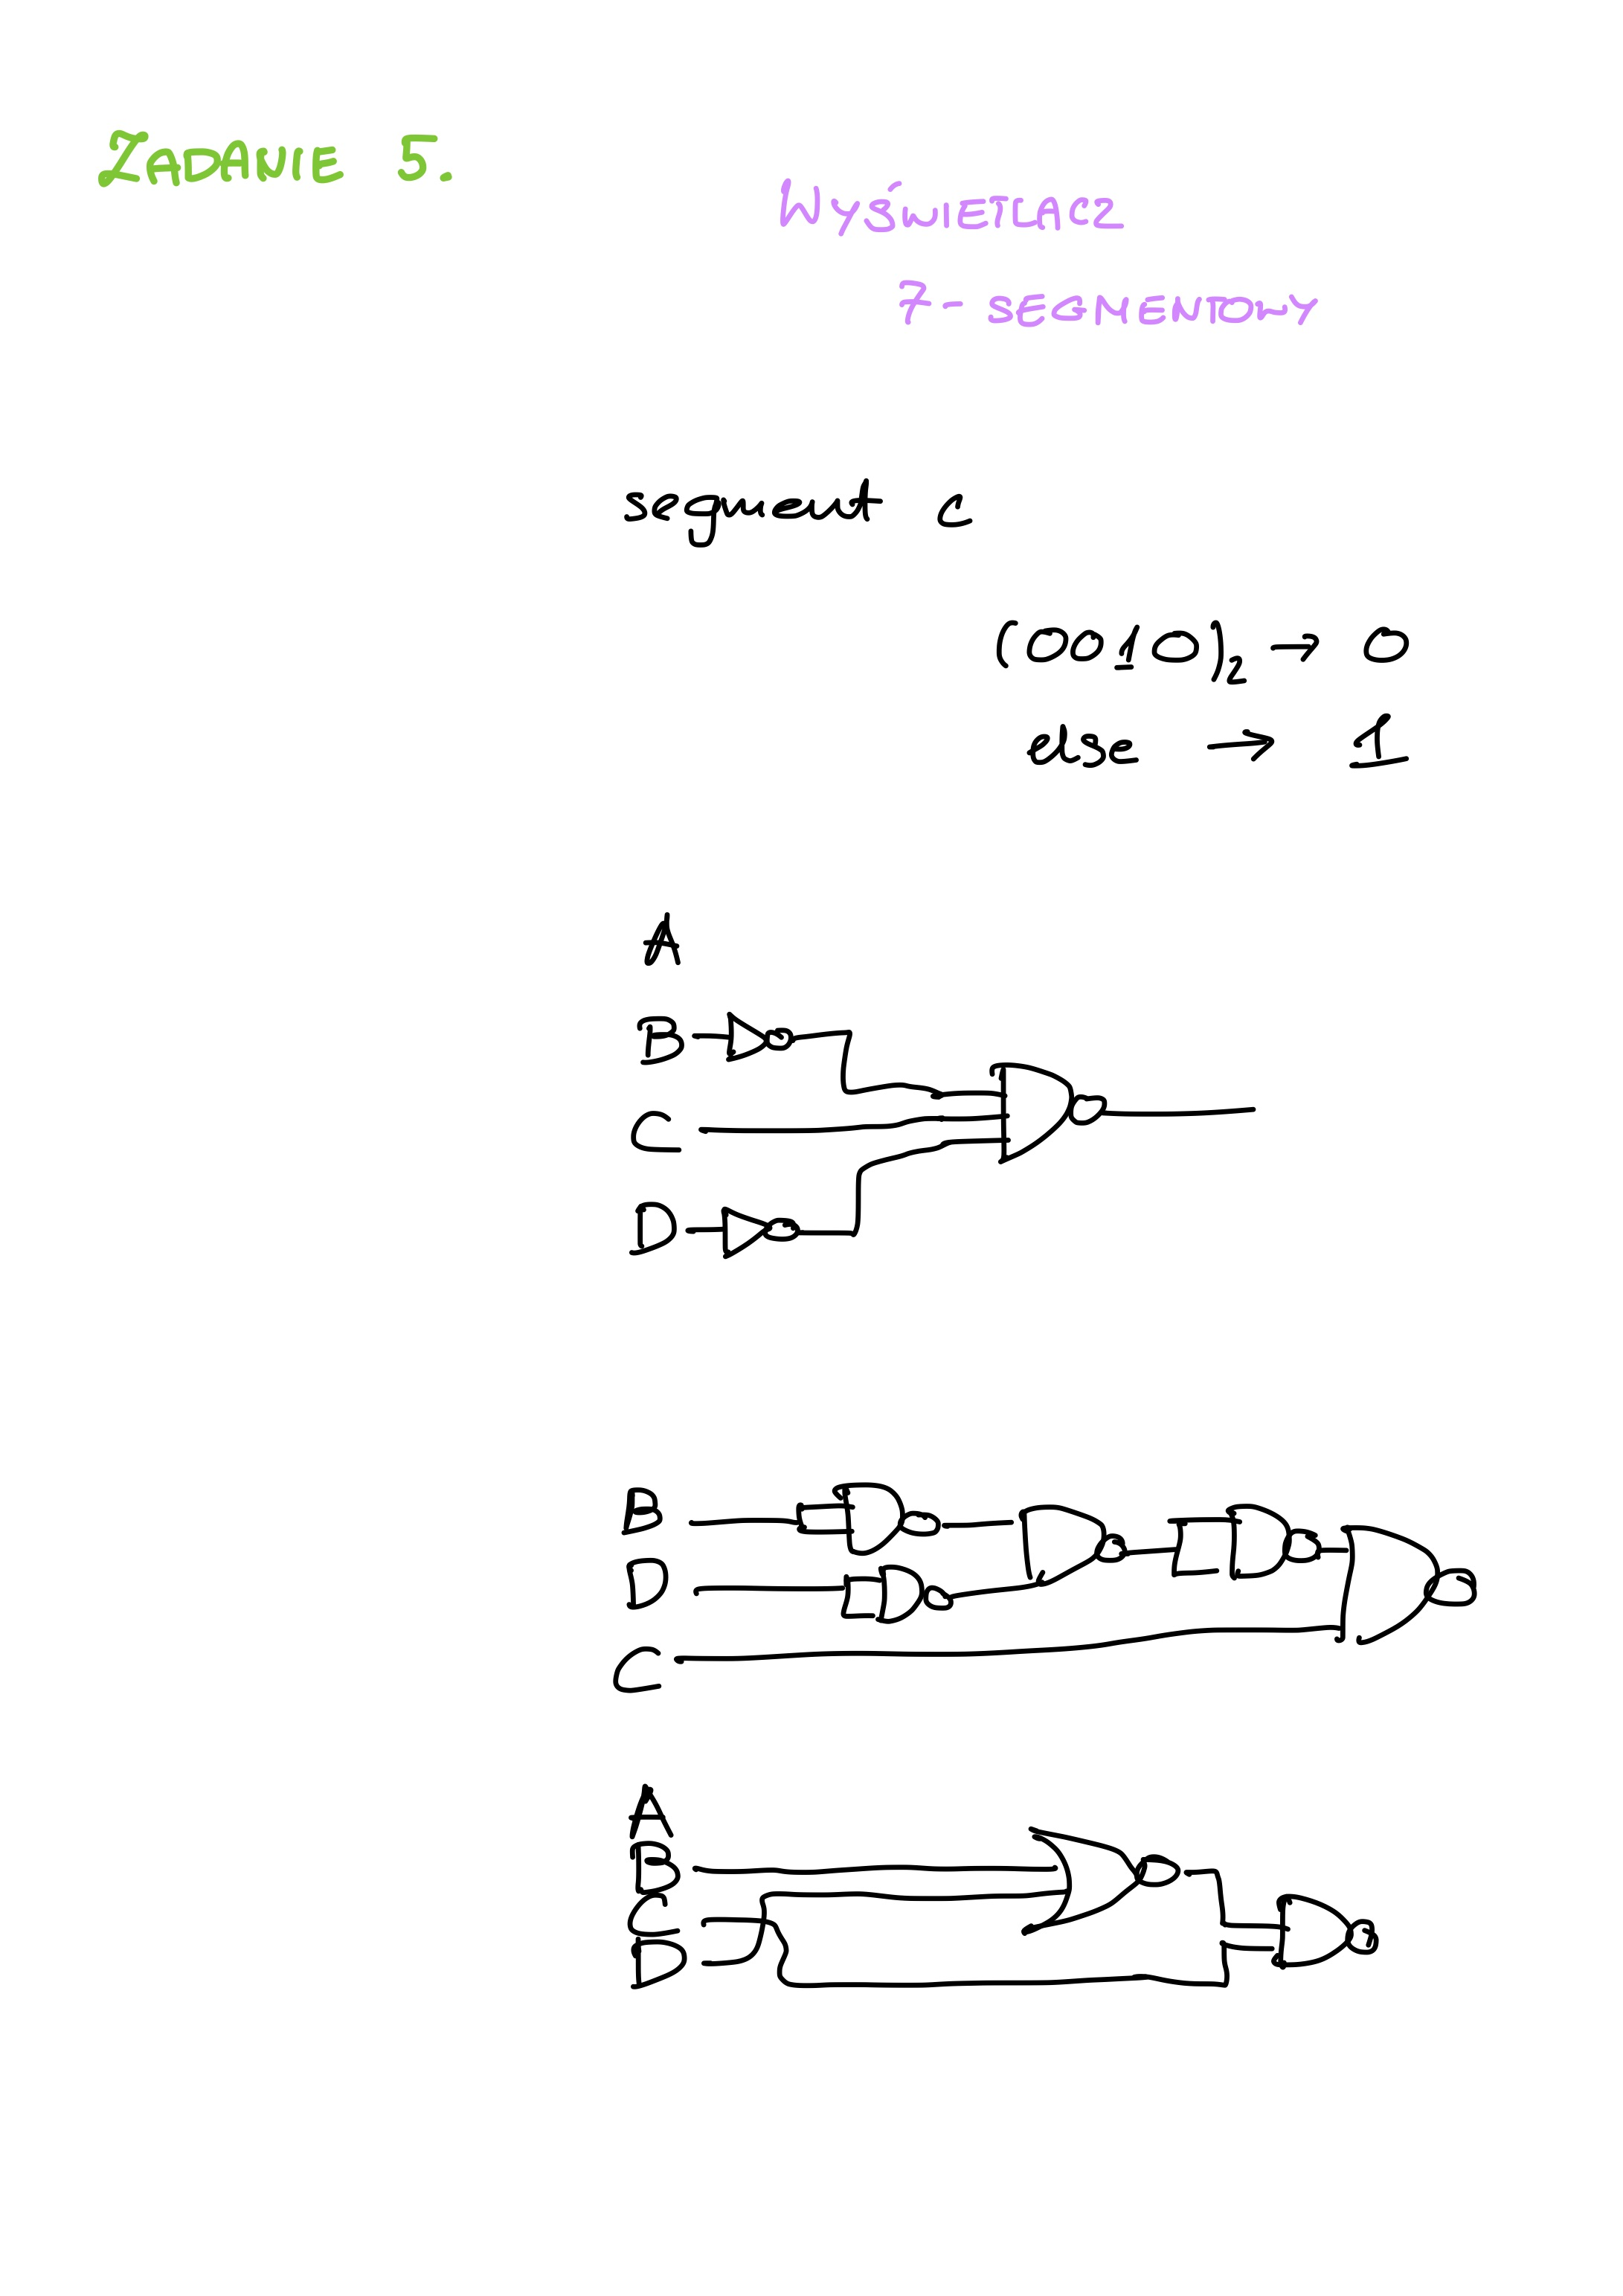
\includegraphics[scale=0.2]{B5}
\centering
\captionsetup{labelformat=empty}
\caption{}
\end{figure}

\begin{figure}[H]
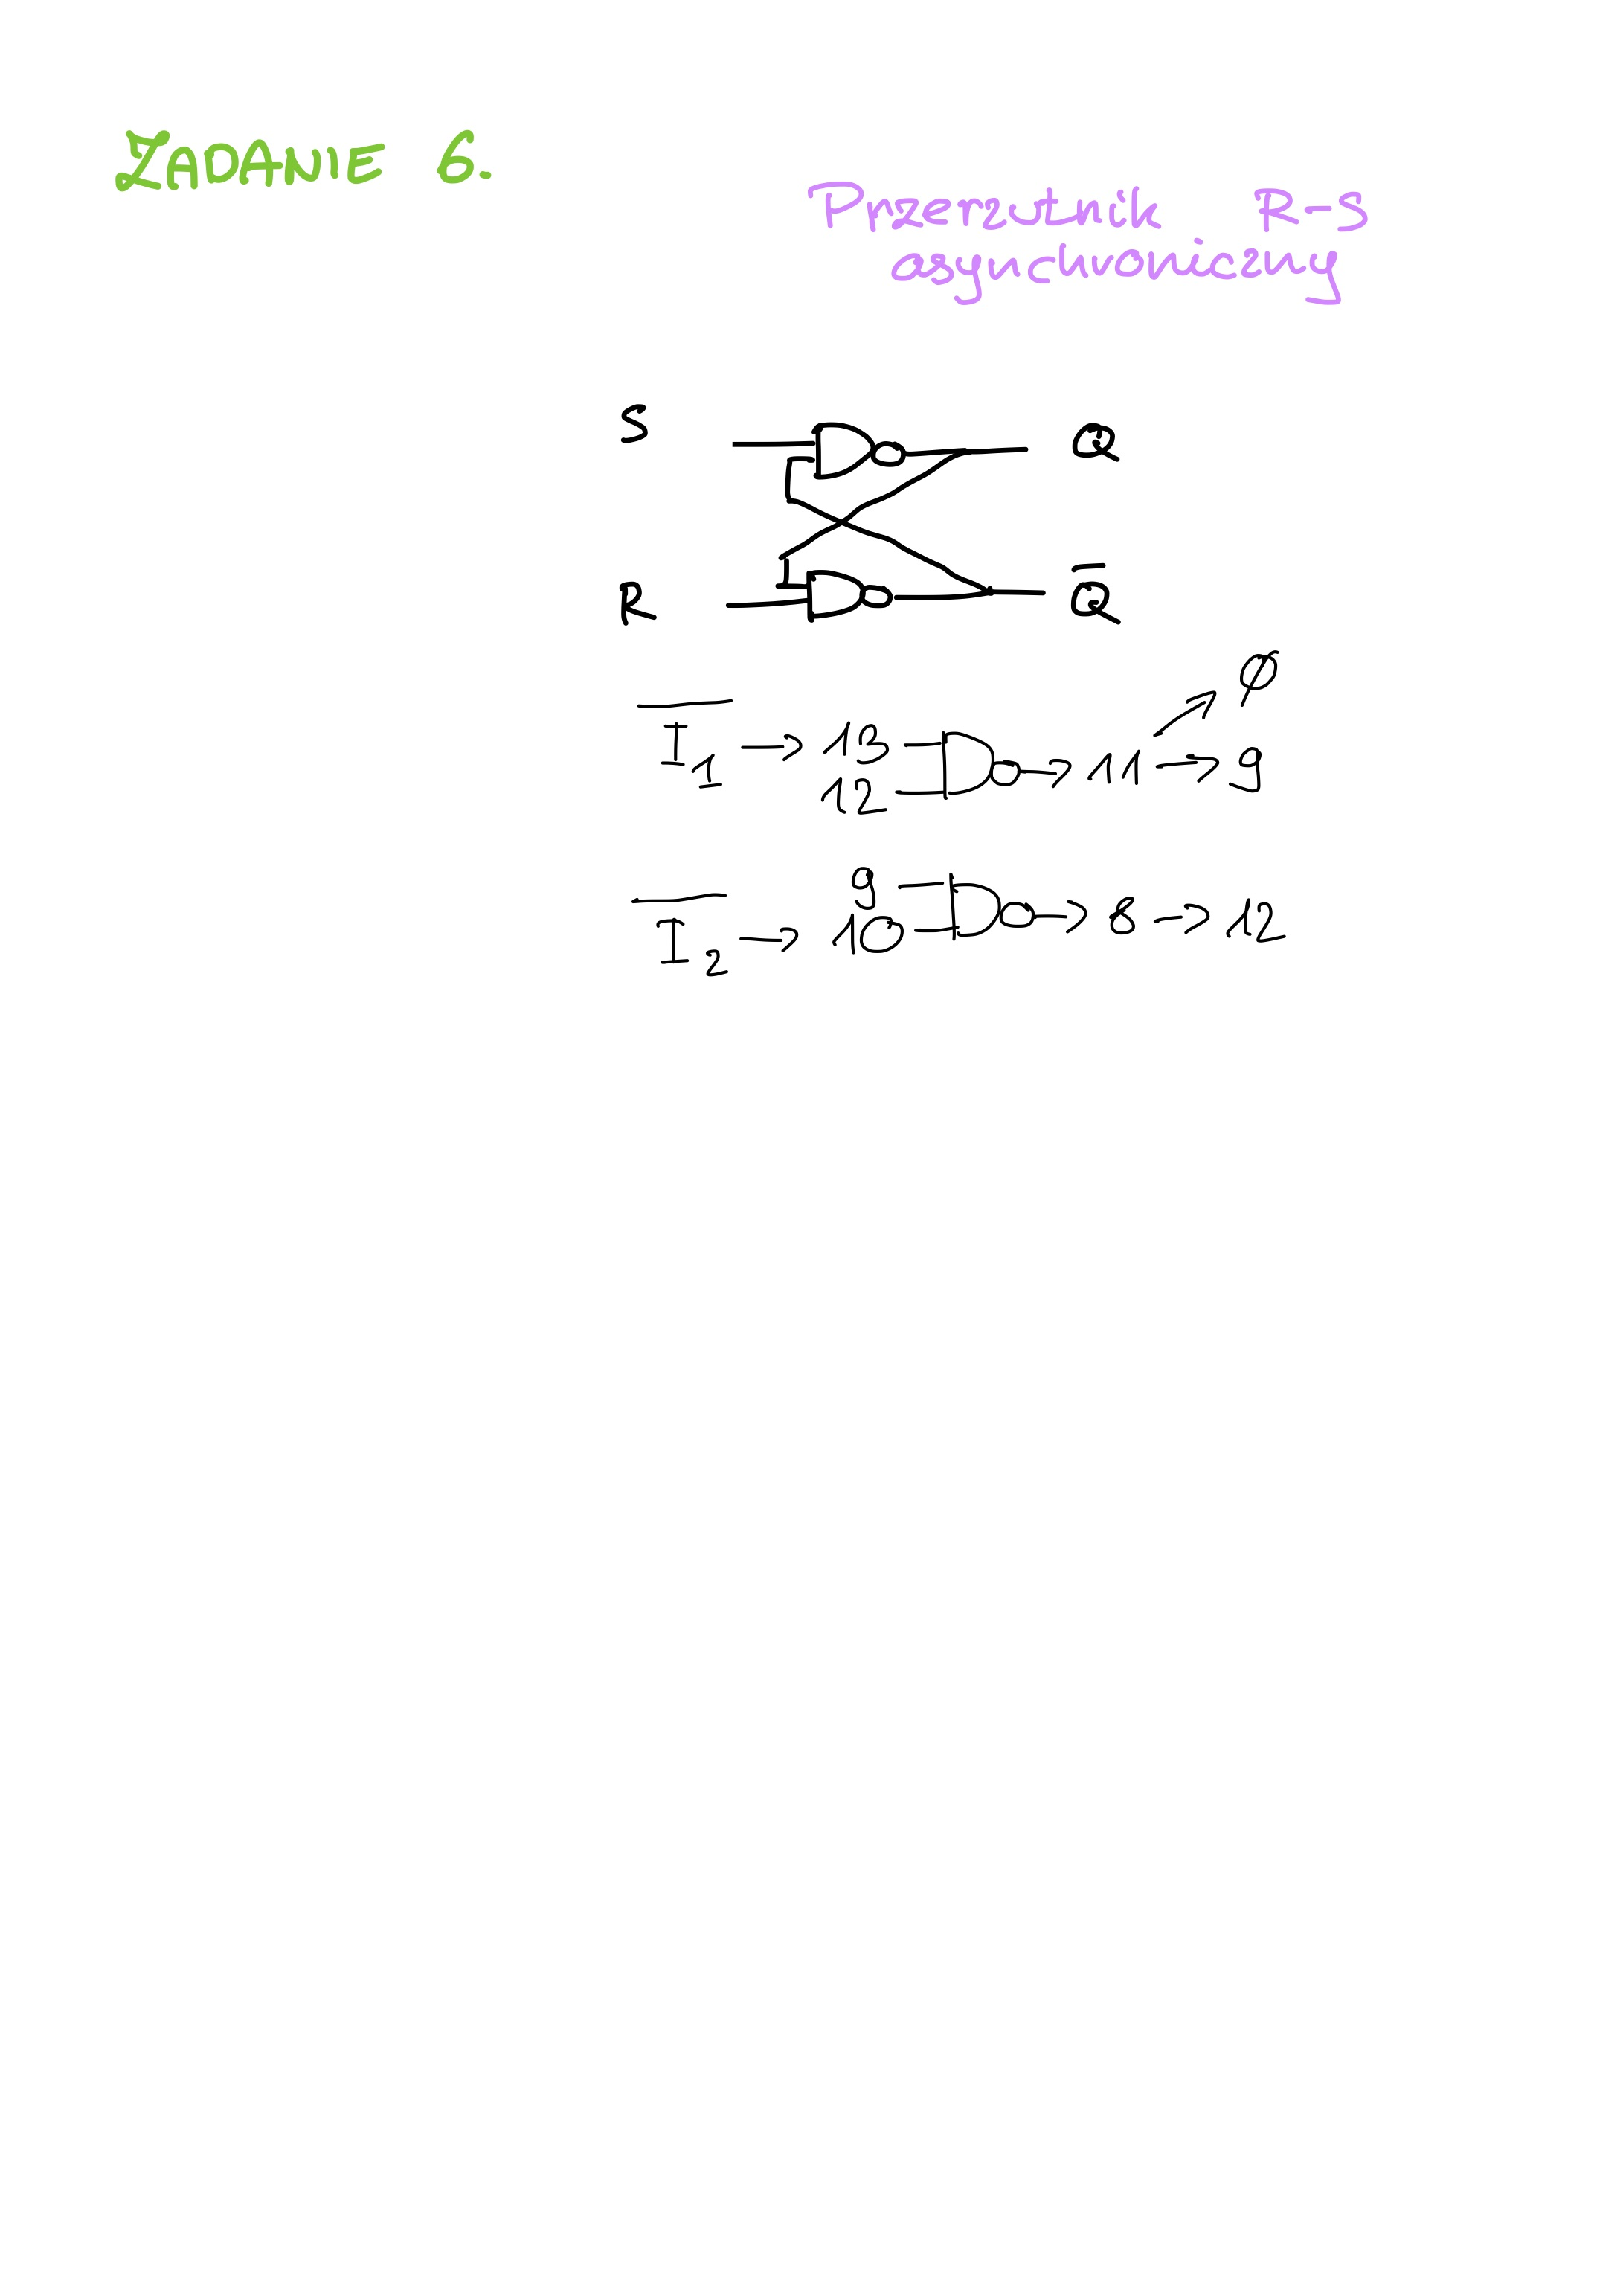
\includegraphics[scale=0.2]{B4}
\centering
\captionsetup{labelformat=empty}
\caption{}
\end{figure}

\end{document}